\documentclass[11pt]{article}

% The four macros of the header standard; tools/zenodo/publish_revision.py patches them when it reserves the DOI.
\newcommand{\doctype}{Preprint}
\newcommand{\docversion}{v1.00.000}
\newcommand{\docdate}{8 November 2026}
\newcommand{\versiondoi}{10.5281/zenodo.24053205}
\newcommand{\conceptdoi}{10.5281/zenodo.24053204}
\newcommand{\docidentity}{CAOS\_Contraste, the validation of the risk models of a bank}

% The packages and conventions every Contraste manuscript shares (CAOS_MANAGE conventions/manuscript-content-bar.md
% section 2). A document sets its class, the four header macros and \docidentity, then % The packages and conventions every Contraste manuscript shares (CAOS_MANAGE conventions/manuscript-content-bar.md
% section 2). A document sets its class, the four header macros and \docidentity, then % The packages and conventions every Contraste manuscript shares (CAOS_MANAGE conventions/manuscript-content-bar.md
% section 2). A document sets its class, the four header macros and \docidentity, then \input{../_shared/preamble}.
\usepackage[T1]{fontenc}
\usepackage[utf8]{inputenc}
\usepackage{lmodern}
\usepackage{microtype}
\usepackage[a4paper,margin=2.5cm]{geometry}
\usepackage{amsmath,amssymb,amsthm,mathtools,bm}
\usepackage{graphicx}
\usepackage{booktabs,longtable,tabularx,array,multirow}
\usepackage{siunitx}
\usepackage{algorithm}
\usepackage{algpseudocode}
\usepackage{caption,subcaption}
\usepackage{xcolor}
\usepackage[numbers,sort&compress]{natbib}
\usepackage[hidelinks]{hyperref}
\usepackage{cleveref}
\usepackage{orcidlink}

\sisetup{group-separator={,},group-minimum-digits=4,detect-all}
\graphicspath{{figures/}{../figures/}}
\captionsetup{font=small,labelfont=bf}
\setlength{\LTcapwidth}{\textwidth}

% Theorem environments for the Theory sections of the manuscripts.
\newtheorem{proposition}{Proposition}
\newtheorem{lemma}{Lemma}
\newtheorem{corollary}{Corollary}
\theoremstyle{definition}
\newtheorem{definition}{Definition}
\newtheorem{assumption}{Assumption}
\theoremstyle{remark}
\newtheorem{remark}{Remark}

% Notation shared by the documents (each defines it again in its notation table).
\newcommand{\E}{\mathbb{E}}
\newcommand{\Prob}{\mathbb{P}}
\newcommand{\Var}{\operatorname{Var}}
\newcommand{\Cov}{\operatorname{Cov}}
\newcommand{\VaR}{\operatorname{VaR}}
\newcommand{\ES}{\operatorname{ES}}
\newcommand{\PD}{\mathrm{PD}}
\newcommand{\LGD}{\mathrm{LGD}}
\newcommand{\EAD}{\mathrm{EAD}}
\newcommand{\ECL}{\mathrm{ECL}}
\newcommand{\indic}{\mathbf{1}}
\newcommand{\R}{\mathbb{R}}
\newcommand{\dd}{\,\mathrm{d}}

% The page-1 header block (CAOS_MANAGE conventions/manuscript-header-standard.md). The document defines \doctype,
% \docversion, \docdate, \versiondoi, \conceptdoi and \docidentity before this file; the publishing tool patches the four
% macros of the standard when it reserves the version DOI.
\newcommand{\docrepo}{github.com/fsantibanezleal/CAOS\_Contraste}
\newcommand{\headerblock}{%
\begin{center}
\fbox{\parbox{0.94\textwidth}{\small\raggedright
\textbf{\doctype} \quad$\cdot$\quad \docversion, \docdate \quad$\cdot$\quad Licence CC BY 4.0\\[2pt]
CAOS open-research programme \quad$\cdot$\quad \docidentity\\[2pt]
Version DOI \href{https://doi.org/\versiondoi}{\texttt{\versiondoi}} \quad$\cdot$\quad
concept DOI (always latest) \href{https://doi.org/\conceptdoi}{\texttt{\conceptdoi}}\\[2pt]
Not peer reviewed. Source code, data and computational records: \href{https://\docrepo}{\texttt{\docrepo}}
}}
\end{center}
\vspace{4pt}}
.
\usepackage[T1]{fontenc}
\usepackage[utf8]{inputenc}
\usepackage{lmodern}
\usepackage{microtype}
\usepackage[a4paper,margin=2.5cm]{geometry}
\usepackage{amsmath,amssymb,amsthm,mathtools,bm}
\usepackage{graphicx}
\usepackage{booktabs,longtable,tabularx,array,multirow}
\usepackage{siunitx}
\usepackage{algorithm}
\usepackage{algpseudocode}
\usepackage{caption,subcaption}
\usepackage{xcolor}
\usepackage[numbers,sort&compress]{natbib}
\usepackage[hidelinks]{hyperref}
\usepackage{cleveref}
\usepackage{orcidlink}

\sisetup{group-separator={,},group-minimum-digits=4,detect-all}
\graphicspath{{figures/}{../figures/}}
\captionsetup{font=small,labelfont=bf}
\setlength{\LTcapwidth}{\textwidth}

% Theorem environments for the Theory sections of the manuscripts.
\newtheorem{proposition}{Proposition}
\newtheorem{lemma}{Lemma}
\newtheorem{corollary}{Corollary}
\theoremstyle{definition}
\newtheorem{definition}{Definition}
\newtheorem{assumption}{Assumption}
\theoremstyle{remark}
\newtheorem{remark}{Remark}

% Notation shared by the documents (each defines it again in its notation table).
\newcommand{\E}{\mathbb{E}}
\newcommand{\Prob}{\mathbb{P}}
\newcommand{\Var}{\operatorname{Var}}
\newcommand{\Cov}{\operatorname{Cov}}
\newcommand{\VaR}{\operatorname{VaR}}
\newcommand{\ES}{\operatorname{ES}}
\newcommand{\PD}{\mathrm{PD}}
\newcommand{\LGD}{\mathrm{LGD}}
\newcommand{\EAD}{\mathrm{EAD}}
\newcommand{\ECL}{\mathrm{ECL}}
\newcommand{\indic}{\mathbf{1}}
\newcommand{\R}{\mathbb{R}}
\newcommand{\dd}{\,\mathrm{d}}

% The page-1 header block (CAOS_MANAGE conventions/manuscript-header-standard.md). The document defines \doctype,
% \docversion, \docdate, \versiondoi, \conceptdoi and \docidentity before this file; the publishing tool patches the four
% macros of the standard when it reserves the version DOI.
\newcommand{\docrepo}{github.com/fsantibanezleal/CAOS\_Contraste}
\newcommand{\headerblock}{%
\begin{center}
\fbox{\parbox{0.94\textwidth}{\small\raggedright
\textbf{\doctype} \quad$\cdot$\quad \docversion, \docdate \quad$\cdot$\quad Licence CC BY 4.0\\[2pt]
CAOS open-research programme \quad$\cdot$\quad \docidentity\\[2pt]
Version DOI \href{https://doi.org/\versiondoi}{\texttt{\versiondoi}} \quad$\cdot$\quad
concept DOI (always latest) \href{https://doi.org/\conceptdoi}{\texttt{\conceptdoi}}\\[2pt]
Not peer reviewed. Source code, data and computational records: \href{https://\docrepo}{\texttt{\docrepo}}
}}
\end{center}
\vspace{4pt}}
.
\usepackage[T1]{fontenc}
\usepackage[utf8]{inputenc}
\usepackage{lmodern}
\usepackage{microtype}
\usepackage[a4paper,margin=2.5cm]{geometry}
\usepackage{amsmath,amssymb,amsthm,mathtools,bm}
\usepackage{graphicx}
\usepackage{booktabs,longtable,tabularx,array,multirow}
\usepackage{siunitx}
\usepackage{algorithm}
\usepackage{algpseudocode}
\usepackage{caption,subcaption}
\usepackage{xcolor}
\usepackage[numbers,sort&compress]{natbib}
\usepackage[hidelinks]{hyperref}
\usepackage{cleveref}
\usepackage{orcidlink}

\sisetup{group-separator={,},group-minimum-digits=4,detect-all}
\graphicspath{{figures/}{../figures/}}
\captionsetup{font=small,labelfont=bf}
\setlength{\LTcapwidth}{\textwidth}

% Theorem environments for the Theory sections of the manuscripts.
\newtheorem{proposition}{Proposition}
\newtheorem{lemma}{Lemma}
\newtheorem{corollary}{Corollary}
\theoremstyle{definition}
\newtheorem{definition}{Definition}
\newtheorem{assumption}{Assumption}
\theoremstyle{remark}
\newtheorem{remark}{Remark}

% Notation shared by the documents (each defines it again in its notation table).
\newcommand{\E}{\mathbb{E}}
\newcommand{\Prob}{\mathbb{P}}
\newcommand{\Var}{\operatorname{Var}}
\newcommand{\Cov}{\operatorname{Cov}}
\newcommand{\VaR}{\operatorname{VaR}}
\newcommand{\ES}{\operatorname{ES}}
\newcommand{\PD}{\mathrm{PD}}
\newcommand{\LGD}{\mathrm{LGD}}
\newcommand{\EAD}{\mathrm{EAD}}
\newcommand{\ECL}{\mathrm{ECL}}
\newcommand{\indic}{\mathbf{1}}
\newcommand{\R}{\mathbb{R}}
\newcommand{\dd}{\,\mathrm{d}}

% The page-1 header block (CAOS_MANAGE conventions/manuscript-header-standard.md). The document defines \doctype,
% \docversion, \docdate, \versiondoi, \conceptdoi and \docidentity before this file; the publishing tool patches the four
% macros of the standard when it reserves the version DOI.
\newcommand{\docrepo}{github.com/fsantibanezleal/CAOS\_Contraste}
\newcommand{\headerblock}{%
\begin{center}
\fbox{\parbox{0.94\textwidth}{\small\raggedright
\textbf{\doctype} \quad$\cdot$\quad \docversion, \docdate \quad$\cdot$\quad Licence CC BY 4.0\\[2pt]
CAOS open-research programme \quad$\cdot$\quad \docidentity\\[2pt]
Version DOI \href{https://doi.org/\versiondoi}{\texttt{\versiondoi}} \quad$\cdot$\quad
concept DOI (always latest) \href{https://doi.org/\conceptdoi}{\texttt{\conceptdoi}}\\[2pt]
Not peer reviewed. Source code, data and computational records: \href{https://\docrepo}{\texttt{\docrepo}}
}}
\end{center}
\vspace{4pt}}

\setlength{\emergencystretch}{3em}
% One macro per number quoted in the prose, written by make_tables.py from the stored results.
% Generated by make_numbers.py and make_tables.py: one macro per number of the prose; the comment names its source.
% results_reverse_c16.json bases.list-adverse.engine.multiplier
\newcommand{\mAdv}{2.118175}
% results_reverse_c16.json bases.list-extreme.engine.multiplier
\newcommand{\mExt}{1.383141}
% results_reverse_c16.json bases.list-adverse.base_sp
\newcommand{\spAdv}{62}
% results_reverse_c16.json bases.list-extreme.base_sp
\newcommand{\spExt}{41}
% results_reverse_c16.json bases.list-adverse.cap
\newcommand{\capAdv}{145.2}
% results_reverse_c16.json bases.list-extreme.cap
\newcommand{\capExt}{93.9}
% results_reverse_c16.json bases.fast-run.cap
\newcommand{\capFast}{18.43}
% results_reverse_c16.json bases.list-adverse.engine.evals
\newcommand{\evalsSolve}{17}
% results_reverse_c16.json bases.list-adverse.time_us_median
\newcommand{\timeAdvMs}{3.8}
% results_reverse_c16.json bases.list-extreme.time_us_median
\newcommand{\timeExtMs}{3.0}
% results_reverse_c16.json bases.list-adverse.hyperbolic_rule.value
\newcommand{\hypAdv}{2.067}
% results_reverse_c16.json bases.list-extreme.hyperbolic_rule.value
\newcommand{\hypExt}{1.367}
% results_reverse_c16.json bases.list-adverse.hyperbolic_rule.rel_error x 100
\newcommand{\hypAdvErr}{2.4}
% results_reverse_c16.json bases.list-extreme.hyperbolic_rule.rel_error x 100
\newcommand{\hypExtErr}{1.2}
% results_reverse_c16.json bases.list-adverse.raw_capacity_multiplier
\newcommand{\rawAdv}{2.194759}
% results_reverse_c16.json bases.list-extreme.raw_capacity_multiplier
\newcommand{\rawExt}{1.433265}
% results_reverse_c16.json raw over engine, adverse, percent
\newcommand{\rawAdvPct}{3.6}
% results_reverse_c16.json derivative.list-adverse.elasticity
\newcommand{\elastAdv}{1.55}
% results_reverse_c16.json derivative.list-adverse.rel_difference x 100
\newcommand{\derivRelAdv}{0.0045}
% results_reverse_c16.json derivative.list-extreme.rel_difference x 100
\newcommand{\derivRelExt}{0.0031}
% results_reverse_c16.json derivative.list-adverse.capacity_at_t0 / 1e6 (USD billion; money in thousands)
\newcommand{\capTzero}{70.1}
% results_reverse_c16.json derivative.list-adverse.t0_day
\newcommand{\dayZeroAdv}{30}
% results_reverse_c16.json band.list-adverse.one_at_a_time haircut low
\newcommand{\hcLowAdv}{2.229711}
% results_reverse_c16.json band.list-adverse.one_at_a_time haircut high
\newcommand{\hcHighAdv}{1.946672}
% results_reverse_c16.json haircut low over central, percent
\newcommand{\hcLowAdvPct}{5.3}
% results_reverse_c16.json haircut high under central, percent
\newcommand{\hcHighAdvPct}{8.1}
% results_reverse_c16.json band.list-adverse.joint_min
\newcommand{\jointMinAdv}{1.063646}
% results_reverse_c16.json band.list-adverse.joint_max
\newcommand{\jointMaxAdv}{2.229711}
% results_reverse_c16.json band.list-adverse.joint_max_rel_deviation x 100
\newcommand{\jointDevAdv}{49.8}
% results_reverse_c16.json band.list-adverse monetisation slow refusal
\newcommand{\slowSpAdv}{4}
% results_reverse_c16.json band.list-extreme monetisation slow refusal
\newcommand{\slowSpExt}{3}
% results_reverse_c16.json band.list-adverse solved combinations of 9
\newcommand{\jointSolvedAdv}{7}
% results_reverse_c16.json band.list-adverse.mapping operational
\newcommand{\opAdv}{2.796956}
% results_reverse_c16.json band.list-adverse.mapping operational base_sp
\newcommand{\opSpAdv}{79}
% results_reverse_c16.json band.list-adverse.mapping other legal entities base_sp
\newcommand{\legalSp}{1}
% results_reverse_c16.json band.list-adverse.uninsured_share[0]
\newcommand{\uninsLowAdv}{2.712}
% results_reverse_c16.json band.list-adverse.uninsured_share[-1]
\newcommand{\uninsHighAdv}{2.105}
% results_reverse_c16.json band.list-adverse.by_target_solved_up_to
\newcommand{\tMaxAdv}{61}
% results_reverse_c16.json band.list-extreme.by_target_solved_up_to
\newcommand{\tMaxExt}{40}
% results_reverse_c16.json labelled_run.svb_modelled_2d
\newcommand{\svbModel}{0.1708}
% results_reverse_c16.json labelled_run.svb_ratio_2d
\newcommand{\svbRatio}{0.201}
% results_reverse_c16.json labelled_run.rows SVB UK modelled
\newcommand{\ukModel}{0.1263}
% results_reverse_c16.json labelled_run.rows SVB UK ratio
\newcommand{\ukRatio}{0.421}
% results_reverse_c16.json labelled_run.rows Signature ratio
\newcommand{\sigRatio}{0.631}
% results_reverse_c16.json labelled_run.rows Northern Rock modelled
\newcommand{\nrModel}{0.2528}
% results_reverse_c16.json labelled_run.rows Northern Rock ratio
\newcommand{\nrRatio}{1.264}
% results_reverse_c16.json labelled_run.denominators call-report-dep ratio
\newcommand{\depRatio}{0.214}
% results_reverse_c16.json labelled_run.denominators call-report-dep realised_share
\newcommand{\depShare}{0.798}
% results_reverse_c16.json labelled_run.rules max
\newcommand{\rateMax}{0.054258}
% results_reverse_c16.json labelled_run.rules median
\newcommand{\rateMed}{0.008209}
% results_reverse_c16.json labelled_run.rules mean
\newcommand{\rateMean}{0.018412}
% results_reverse_c16.json labelled_run.rules median ratio
\newcommand{\medRatio}{0.110}
% results_reverse_c16.json labelled_run.rules mean ratio
\newcommand{\meanRatio}{0.131}
% results_reverse_c16.json labelled_run.leave_one_out Northern Rock
\newcommand{\looNr}{0.010481}
% results_reverse_c16.json labelled_run.multiplier_of_labelled_run
\newcommand{\mSvb}{12.22}
% results_reverse_c16.json labelled_run.reverse_by_target.2.multiplier
\newcommand{\mTwo}{2.669936}
% results_reverse_c16.json labelled_run.reverse_by_target.4.multiplier
\newcommand{\mFour}{2.06764}
% results_reverse_c16.json labelled_run.reverse_by_target.2.sp_just_below
\newcommand{\spBelowTwo}{4}
% results_reverse_c16.json labelled_run.ratio_labelled_to_reverse_t2
\newcommand{\ratioLab}{4.58}
% results_reverse_c16.json labelled_run.opening_total / 1e6 (USD billion)
\newcommand{\svbAdvTotal}{175.5}
% results_theory.json monotone_in_multiplier.comparisons
\newcommand{\thMonoCmp}{117,000}
% results_theory.json monotone_in_multiplier.banks
\newcommand{\thMonoBanks}{3,000}
% results_theory.json closed_form_single_segment.instances
\newcommand{\thCfN}{3,000}
% results_theory.json closed_form_single_segment.solved
\newcommand{\thCfSolved}{1,953}
% results_theory.json closed_form_single_segment.max_abs_difference x 1e6
\newcommand{\thCfMax}{1.000}
% results_theory.json closed_form_single_segment.median_abs_difference x 1e6
\newcommand{\thCfMed}{0.508}
% results_theory.json closed_form_single_segment.hyperbolic_instances
\newcommand{\thHypN}{983}
% results_theory.json hyperbolic_relative_error_median x 100
\newcommand{\thHypMed}{2.0}
% results_theory.json hyperbolic_relative_error_q90 x 100
\newcommand{\thHypQninety}{8.3}
% results_theory.json monotone_in_target.pairs
\newcommand{\thTgtPairs}{2,152}
% results_theory.json monotone_in_capacity.pairs
\newcommand{\thCapPairs}{626}
% results_theory.json exact_round_trip.solved_flat_no_inflow
\newcommand{\thErN}{710}
% results_theory.json exact_round_trip.margin_min
\newcommand{\thErMarginMin}{787}
% results_corpus.json design.instances
\newcommand{\kInst}{20,000}
% results_corpus.json design banks_per_seed x seeds
\newcommand{\kBanks}{5,000}
% results_corpus.json design.instances - design.solved
\newcommand{\kRefused}{11,432}
% results_corpus.json design.solved
\newcommand{\kSolved}{8,568}
% results_corpus.json design.refused_horizon
\newcommand{\kHor}{5,034}
% results_corpus.json design.refused_base
\newcommand{\kBase}{5,870}
% results_corpus.json design.refused_unreachable
\newcommand{\kUnr}{528}
% results_corpus.json design.solved_flat_no_inflow
\newcommand{\kFlat}{2,318}
% results_corpus.json design.solved_growing
\newcommand{\kGrow}{5,177}
% results_corpus.json design.wall_seconds_total / 60
\newcommand{\kWallMin}{30}
% results_corpus.json platform.processor
\newcommand{\kProc}{Intel64 Family 6 Model 183 Stepping 1, GenuineIntel}
% results_corpus.json platform.python
\newcommand{\kPy}{3.13.14}
% results_corpus.json methods.proposed.false_answer_on_refused
\newcommand{\kPFalse}{0.0 (0.0 to 0.0)}
% results_corpus.json methods.proposed.false_answer_on_refused.k
\newcommand{\kPFalseK}{0}
% results_corpus.json methods.proposed.miss_on_solved
\newcommand{\kPMiss}{0.0 (0.0 to 0.0)}
% results_corpus.json methods.proposed.miss_on_solved.k
\newcommand{\kPMissK}{0}
% results_corpus.json methods.proposed.threshold_property_on_solved
\newcommand{\kPThr}{100.0 (100.0 to 100.0)}
% results_corpus.json methods.proposed.answered_beyond_cap
\newcommand{\kPBeyond}{0.0 (0.0 to 0.0)}
% results_corpus.json methods.proposed.abs_rel_error_median
\newcommand{\kPErr}{8.88e-08}
% results_corpus.json methods.proposed.abs_rel_error_median x 100
\newcommand{\kPErrPc}{0.0}
% results_corpus.json methods.proposed.abs_rel_error_q95
\newcommand{\kPErrQ}{0.000}
% results_corpus.json methods.proposed.evals_mean_solved
\newcommand{\kPEvals}{15.7}
% results_corpus.json methods.proposed.time_us_median / 1000 (ms)
\newcommand{\kPTime}{0.29}
% results_corpus.json methods.grid_case.false_answer_on_refused
\newcommand{\kGFalse}{93.5 (93.0 to 93.9)}
% results_corpus.json methods.grid_case.false_answer_on_refused.k
\newcommand{\kGFalseK}{10,684}
% results_corpus.json methods.grid_case.miss_on_solved
\newcommand{\kGMiss}{3.1 (2.7 to 3.4)}
% results_corpus.json methods.grid_case.miss_on_solved.k
\newcommand{\kGMissK}{262}
% results_corpus.json methods.grid_case.threshold_property_on_solved
\newcommand{\kGThr}{0.0 (0.0 to 0.0)}
% results_corpus.json methods.grid_case.answered_beyond_cap
\newcommand{\kGBeyond}{0.0 (0.0 to 0.0)}
% results_corpus.json methods.grid_case.abs_rel_error_median
\newcommand{\kGErr}{2.17e-01}
% results_corpus.json methods.grid_case.abs_rel_error_median x 100
\newcommand{\kGErrPc}{21.7}
% results_corpus.json methods.grid_case.abs_rel_error_q95
\newcommand{\kGErrQ}{0.574}
% results_corpus.json methods.grid_case.evals_mean_solved
\newcommand{\kGEvals}{9.7}
% results_corpus.json methods.grid_case.time_us_median / 1000 (ms)
\newcommand{\kGTime}{1.88}
% results_corpus.json methods.grid_fine.false_answer_on_refused
\newcommand{\kFFalse}{93.7 (93.3 to 94.1)}
% results_corpus.json methods.grid_fine.false_answer_on_refused.k
\newcommand{\kFFalseK}{10,713}
% results_corpus.json methods.grid_fine.miss_on_solved
\newcommand{\kFMiss}{1.4 (1.2 to 1.7)}
% results_corpus.json methods.grid_fine.miss_on_solved.k
\newcommand{\kFMissK}{119}
% results_corpus.json methods.grid_fine.threshold_property_on_solved
\newcommand{\kFThr}{0.0 (0.0 to 0.0)}
% results_corpus.json methods.grid_fine.answered_beyond_cap
\newcommand{\kFBeyond}{0.0 (0.0 to 0.0)}
% results_corpus.json methods.grid_fine.abs_rel_error_median
\newcommand{\kFErr}{1.34e-02}
% results_corpus.json methods.grid_fine.abs_rel_error_median x 100
\newcommand{\kFErrPc}{1.3}
% results_corpus.json methods.grid_fine.abs_rel_error_q95
\newcommand{\kFErrQ}{0.286}
% results_corpus.json methods.grid_fine.evals_mean_solved
\newcommand{\kFEvals}{171.6}
% results_corpus.json methods.grid_fine.time_us_median / 1000 (ms)
\newcommand{\kFTime}{35.14}
% results_corpus.json methods.brent_sp.false_answer_on_refused
\newcommand{\kBFalse}{13.5 (12.9 to 14.2)}
% results_corpus.json methods.brent_sp.false_answer_on_refused.k
\newcommand{\kBFalseK}{1,545}
% results_corpus.json methods.brent_sp.miss_on_solved
\newcommand{\kBMiss}{0.0 (0.0 to 0.0)}
% results_corpus.json methods.brent_sp.miss_on_solved.k
\newcommand{\kBMissK}{0}
% results_corpus.json methods.brent_sp.threshold_property_on_solved
\newcommand{\kBThr}{15.7 (14.9 to 16.4)}
% results_corpus.json methods.brent_sp.answered_beyond_cap
\newcommand{\kBBeyond}{0.0 (0.0 to 0.0)}
% results_corpus.json methods.brent_sp.abs_rel_error_median
\newcommand{\kBErr}{6.35e-02}
% results_corpus.json methods.brent_sp.abs_rel_error_median x 100
\newcommand{\kBErrPc}{6.3}
% results_corpus.json methods.brent_sp.abs_rel_error_q95
\newcommand{\kBErrQ}{0.642}
% results_corpus.json methods.brent_sp.evals_mean_solved
\newcommand{\kBEvals}{15.0}
% results_corpus.json methods.brent_sp.time_us_median / 1000 (ms)
\newcommand{\kBTime}{0.30}
% results_corpus.json methods.bisect_no_refusal.false_answer_on_refused
\newcommand{\kNFalse}{100.0 (100.0 to 100.0)}
% results_corpus.json methods.bisect_no_refusal.false_answer_on_refused.k
\newcommand{\kNFalseK}{11,432}
% results_corpus.json methods.bisect_no_refusal.miss_on_solved
\newcommand{\kNMiss}{0.0 (0.0 to 0.0)}
% results_corpus.json methods.bisect_no_refusal.miss_on_solved.k
\newcommand{\kNMissK}{0}
% results_corpus.json methods.bisect_no_refusal.threshold_property_on_solved
\newcommand{\kNThr}{99.0 (98.7 to 99.2)}
% results_corpus.json methods.bisect_no_refusal.answered_beyond_cap
\newcommand{\kNBeyond}{3.5 (3.2 to 3.7)}
% results_corpus.json methods.bisect_no_refusal.abs_rel_error_median
\newcommand{\kNErr}{9.22e-08}
% results_corpus.json methods.bisect_no_refusal.abs_rel_error_median x 100
\newcommand{\kNErrPc}{0.0}
% results_corpus.json methods.bisect_no_refusal.abs_rel_error_q95
\newcommand{\kNErrQ}{0.000}
% results_corpus.json methods.bisect_no_refusal.evals_mean_solved
\newcommand{\kNEvals}{61.4}
% results_corpus.json methods.bisect_no_refusal.time_us_median / 1000 (ms)
\newcommand{\kNTime}{2.97}
% results_corpus.json methods.uncapped.false_answer_on_refused
\newcommand{\kUFalse}{4.6 (4.2 to 5.0)}
% results_corpus.json methods.uncapped.false_answer_on_refused.k
\newcommand{\kUFalseK}{528}
% results_corpus.json methods.uncapped.miss_on_solved
\newcommand{\kUMiss}{0.0 (0.0 to 0.0)}
% results_corpus.json methods.uncapped.miss_on_solved.k
\newcommand{\kUMissK}{0}
% results_corpus.json methods.uncapped.threshold_property_on_solved
\newcommand{\kUThr}{65.7 (64.7 to 66.7)}
% results_corpus.json methods.uncapped.answered_beyond_cap
\newcommand{\kUBeyond}{2.0 (1.9 to 2.3)}
% results_corpus.json methods.uncapped.abs_rel_error_median
\newcommand{\kUErr}{2.34e-07}
% results_corpus.json methods.uncapped.abs_rel_error_median x 100
\newcommand{\kUErrPc}{0.0}
% results_corpus.json methods.uncapped.abs_rel_error_q95
\newcommand{\kUErrQ}{0.845}
% results_corpus.json methods.uncapped.evals_mean_solved
\newcommand{\kUEvals}{82.0}
% results_corpus.json methods.uncapped.time_us_median / 1000 (ms)
\newcommand{\kUTime}{0.10}
% results_corpus.json methods.nearest.false_answer_on_refused
\newcommand{\kRFalse}{0.0 (0.0 to 0.0)}
% results_corpus.json methods.nearest.false_answer_on_refused.k
\newcommand{\kRFalseK}{0}
% results_corpus.json methods.nearest.miss_on_solved
\newcommand{\kRMiss}{0.0 (0.0 to 0.0)}
% results_corpus.json methods.nearest.miss_on_solved.k
\newcommand{\kRMissK}{0}
% results_corpus.json methods.nearest.threshold_property_on_solved
\newcommand{\kRThr}{51.1 (50.0 to 52.1)}
% results_corpus.json methods.nearest.answered_beyond_cap
\newcommand{\kRBeyond}{0.0 (0.0 to 0.0)}
% results_corpus.json methods.nearest.abs_rel_error_median
\newcommand{\kRErr}{4.59e-08}
% results_corpus.json methods.nearest.abs_rel_error_median x 100
\newcommand{\kRErrPc}{0.0}
% results_corpus.json methods.nearest.abs_rel_error_q95
\newcommand{\kRErrQ}{0.000}
% results_corpus.json methods.nearest.evals_mean_solved
\newcommand{\kREvals}{8.7}
% results_corpus.json methods.nearest.time_us_median / 1000 (ms)
\newcommand{\kRTime}{0.07}
% results_corpus.json methods.raw_capacity.false_answer_on_refused
\newcommand{\kWFalse}{1.4 (1.2 to 1.6)}
% results_corpus.json methods.raw_capacity.false_answer_on_refused.k
\newcommand{\kWFalseK}{156}
% results_corpus.json methods.raw_capacity.miss_on_solved
\newcommand{\kWMiss}{4.6 (4.2 to 5.1)}
% results_corpus.json methods.raw_capacity.miss_on_solved.k
\newcommand{\kWMissK}{396}
% results_corpus.json methods.raw_capacity.threshold_property_on_solved
\newcommand{\kWThr}{34.4 (33.4 to 35.5)}
% results_corpus.json methods.raw_capacity.answered_beyond_cap
\newcommand{\kWBeyond}{0.0 (0.0 to 0.0)}
% results_corpus.json methods.raw_capacity.abs_rel_error_median
\newcommand{\kWErr}{1.51e-02}
% results_corpus.json methods.raw_capacity.abs_rel_error_median x 100
\newcommand{\kWErrPc}{1.5}
% results_corpus.json methods.raw_capacity.abs_rel_error_q95
\newcommand{\kWErrQ}{0.388}
% results_corpus.json methods.raw_capacity.evals_mean_solved
\newcommand{\kWEvals}{15.0}
% results_corpus.json methods.raw_capacity.time_us_median / 1000 (ms)
\newcommand{\kWTime}{0.31}
% results_corpus.json H1.disagreements
\newcommand{\kHOneDis}{0}
% results_corpus.json H2.diff_min x 1e6
\newcommand{\kHTwoMin}{0.000}
% results_corpus.json H2.diff_max x 1e6
\newcommand{\kHTwoMax}{1.000}
% results_corpus.json H3.monotone
\newcommand{\kHThreeMono}{100.0 (99.8 to 100.0)}
% results_corpus.json H3.growing
\newcommand{\kHThreeGrow}{28.9 (27.6 to 30.1)}
% results_corpus.json H3.gap quantile 0.9
\newcommand{\kHThreeGapNine}{6}
% results_corpus.json H3.gap quantile 0.5
\newcommand{\kHThreeGapFifty}{0}
% results_corpus.json H3.gap max
\newcommand{\kHThreeGapMax}{29}
% results_corpus.json H4
\newcommand{\kHFour}{75.7 (74.8 to 76.7)}
% results_corpus.json H4.overshoot median x 100
\newcommand{\kHFourMed}{21.7}
% results_corpus.json H4.overshoot q90 x 100
\newcommand{\kHFourQ}{51.9}
% results_corpus.json H5.rate_of_all_solved x 100
\newcommand{\kHFive}{82.6}
% results_corpus.json H6
\newcommand{\kHSix}{42.7 (40.2 to 45.2)}
% results_corpus.json H6 median x 100
\newcommand{\kHSixMed}{13.0}
% results_corpus.json raw_capacity_on_flows.median_abs_rel_error x 100
\newcommand{\kRawFlows}{6.5}
% results_corpus.json raw_capacity_on_flows.n
\newcommand{\kRawFlowsN}{5,221}
% results_corpus.json m0_quantiles 0.5
\newcommand{\kMzeroMed}{4.30}
% results_corpus.json m0_quantiles 0.05
\newcommand{\kMzeroLo}{1.17}
% results_corpus.json m0_quantiles 0.95
\newcommand{\kMzeroHi}{38.1}


\title{Reverse liquidity stress as a run-off multiplier with a refusal rule, scored against a labelled run}
\author{Felipe Santib\'a\~nez-Leal~\orcidlink{0000-0002-0150-3246}\\
\small CAOS open-research programme, Santiago, Chile\\
\small \texttt{fsantibanez@gmail.com}}
\date{\docdate}

\begin{document}
\maketitle
\headerblock

\begin{abstract}
Validating a liquidity stress model needs the inverse of the forward scenario: the run-off speed at which a stated survival period is reached.
We define the reverse liquidity stress as the smallest multiplier on the daily run-off rates, capped so that no rate exceeds one, at which the survival period is at most a target.
It is the root of a continuous window function, rounded up with a neighbour check; a target that no multiplier brackets is refused with its reason and no number.
Seven propositions with proofs give its monotonicity, refusal rule, exact round trip and sensitivity.
On \kInst{} seeded instances the engine agrees with an independent oracle on every outcome and returns a threshold on every solved one; a case-grid scan answers \kGFalse{}\,\% of the refused instances and overshoots by a median of \kGErrPc{}\,\%.
On case C16 the multiplier for 30 days is \mAdv{} (LiST Adverse) and \mExt{} (LiST Extreme), and the 2023 fast-run base is refused.
Calibrated on rows before 2023, that base models \svbModel{} of deposits in the two days of the March 2023 run against 0.85 observed (ratio \svbRatio{}), and the multiplier that reproduces the run is \mSvb{} times the calibrated rate.
The Adverse multiplier moves by \jointDevAdv{}\,\% over the joint band of case conventions: under the slow monetisation schedule it is refused at the central haircut and falls to \lowSlowM{} at the low haircut.
Nine of twelve predictions held; three failed.
The bank's deposit behaviour is synthetic.
\end{abstract}

\section{Introduction}
\label{sec:introduction}

A bank that validates its liquidity stress model against the failure of Silicon Valley Bank meets two numbers that do not fit together. The Basel liquidity coverage ratio assumes that deposits leave at rates between 3\% and 40\% over thirty days, and the supervisory stress test of the European Central Bank compounds a small daily rate over six months so that the median survival period of 103 banks is 176 days under its Adverse shock and 122 days under its Extreme shock \citep{bcbs238,ecblist2019,ecbannex2019}. The bank that failed on 10 March 2023 lost about 85\% of its deposits in two days, and the Federal Reserve's review records outflows of more than 40 billion US dollars on 9 March with another 100 billion expected the next day \citep{bcbs555,fedsvb2023}. Both families of assumptions are forward scenarios: they fix a run-off speed and report what the bank survives. A validator who has to say how far a stated scenario is from failure needs the inverse statement, the speed at which the bank just reaches a stated survival period.

That inverse statement is a reverse stress test. The stress-testing principles of the Basel Committee and the literature on reverse tests treat it as a search for the scenario that produces a stated outcome \citep{bcbs155,glasserman2015,breuercsiszar2013,grundke2018}. For liquidity the outcome is the survival period, the first day on which the net liquidity position turns negative, and the search variable that the forward scenarios already share is the speed of the run-off. We study the simplest scenario family that keeps the structure of a supervisory stress: a multiplier $m$ applied to every daily run-off rate of a base scenario, capped so that no rate exceeds one. The reverse stress asks for the smallest multiplier at which the survival period is at most a target of $T$ days.

Three difficulties make the inverse less trivial than the forward calculation. The survival period is an integer day and a bank that never turns negative has no survival period at all, so the function to invert is a step function with a point at infinity. A target that the base scenario already reaches, a target that lies beyond the horizon of the ladder, and a target that no admissible multiplier reaches have no multiplier, and a solver that returns a number for them returns a wrong one. And a multiplier that is reported has to be reproducible: the survival period at the reported value must be the target or lower, and just below it must be longer.

We propose a solver and a measurement protocol that answer these three points. The proposed method defines the reverse stress as the root of a continuous window function of the multiplier, the minimum of the net liquidity position over the first $T$ days; it rounds the root up to six decimals and verifies the threshold property on the neighbouring decimal; and it refuses a target that is not bracketed, with the reason and without a number. The protocol scores a fast-run base, calibrated only on observed runs dated before 2023, against the 2023 rows of the Basel Committee's table of deposit outflows, with the observation of the failed bank as a labelled anchor and never as a forecast \citep{bcbs555}.

The contributions are as follows.
\begin{itemize}
\item A definition of the reverse liquidity stress as a threshold of a continuous, non-increasing window function, with the cap and the rounding rule that make the answer a reproducible number or an explicit refusal (\cref{sec:proposed-method}).
\item Seven propositions with proofs: the monotonicity of the position in the multiplier, the characterisation of the threshold, the soundness and completeness of the refusal rule, a closed form for one segment, an exact round trip with an explicit sufficient condition, two-sided bounds of a hyperbolic approximation, and an implicit-function sensitivity formula (\cref{sec:theory}).
\item A measurement on \kInst{} instances of a seeded corpus of synthetic banks against an independent oracle, with a scan of a fixed multiplier grid, a scan of a fine grid, Brent's method on the survival period and a bisection without the refusal rule as comparators, and an ablation of each component (\cref{sec:results,sec:ablation}).
\item An application to the three committed bases of case C16, a bank whose balance-sheet aggregates are real and whose deposit behaviour is synthetic: the multipliers, their sensitivity to the case conventions, and a score against the run of March 2023 that is red and that we report as such (\cref{sec:results}).
\end{itemize}

The main results are these. On the corpus the proposed solver agrees with the oracle on every instance: it answers none of the \kRefused{} refused instances and misses none of the \kSolved{} solved ones, and every multiplier it returns is a threshold, whereas a scan of the multiplier grid of the case design answers \kGFalse{}\,\% of the refused instances and overshoots the threshold by a median of \kGErrPc{}\,\% in relative terms. On the bank of case C16 the multiplier that brings the survival period to 30 days is \mAdv{} on the Adverse base and \mExt{} on the Extreme base, and the target is refused on the 2023 fast-run base because its ladder is five days long. The fast-run base reproduces \svbRatio{} of the observed two-day outflow of the failed bank, and the multiplier that would reproduce it is \mSvb{} times the calibrated rate. Three of twelve predictions failed, among them the stability of the Adverse multiplier over the joint band of case conventions.

\section{Related work}
\label{sec:related-work}

\subsection{Runs and the speed at which deposits leave}

The theory of deposit runs starts from the observation that a demand-deposit contract gives depositors liquidity and also admits an equilibrium in which all of them withdraw at once \citep{diamond1983}. \citet{goldsteinpauzner2005} make fundamentals decide which equilibrium occurs, which lets them compute the ex ante probability of a panic-based run and relate it to the contract. Both works explain why a run can happen; neither says how fast deposits leave, which is the quantity a liquidity stress test needs. Depositor-level evidence supplies it in part: \citet{iyerpuri2012} follow the depositors of a bank that faced a run and find that uninsured depositors are the most likely to run, that deposit insurance helps only partially, that relationships with the bank mitigate the run and that social networks matter. \citet{cipriani2024} trace the deposit flows of March 2023 from high-frequency interbank payments, identify twenty-two banks that suffered a run, and find that large institutional depositors drove it, that coordination mattered, and that banks that survived a run did so by borrowing new funds and raising deposit rates rather than by selling liquid securities. % voice-ok: withdraw is the depositors action in a bank run, not a version narrative

The funding side of the balance sheet has its own literature. \citet{brunnermeierpedersen2009} model the link between the market liquidity of an asset and the funding liquidity of traders, and show that under certain conditions margins are destabilising and the two reinforce each other in liquidity spirals; \citet{drehmannnikolaou2013} define funding liquidity as the ability to settle obligations with immediacy and propose a measure of its risk built on bids at central bank auctions; \citet{gortonmetrick2012} argue that the panic of 2007 to 2008 was a run on the repo market, with securitised banking at its centre, and document it with the credit spreads of securitised bonds and repo rates; and \citet{acharyamora2015} document that at the onset of the 2007 to 2009 crisis aggregate deposit inflows weakened and loan-to-deposit shortfalls widened, most at banks with greater undrawn commitments. These works explain why funding dries up and where it is fragile; none gives the speed of outflow at which a stated buffer is exhausted. \citet{tirole2011} reviews illiquidity and explains why liquidity cannot easily be apprehended through a single statistic, which is the reason the reverse stress below is stated for a survival period under a stated scenario and not as a general liquidity measure. For 2023, \citet{jiang2024} mark the assets of United States banks to market after the rise in interest rates and examine the role of unrealised losses and uninsured depositors in the runs; they report an average decline of about 10\% in the value of bank assets, about 2 trillion US dollars in aggregate. \citet{cookson2026} study social media as a catalyst of the run on the failed bank; their working-paper abstract reports that banks with high pre-run exposure to Twitter lost more stock market value during the run, and we have not checked the figures of the published version. In the abstract of the working paper under its first title, ``Banking on Uninsured Deposits'',\citet{drechsler2023} show that a run equilibrium among uninsured depositors is absent at low interest rates and appears when rates rise, because the deposit franchise then dominates the value of the bank, so that the liquidity risk of a bank increases with interest rates. What these studies imply for a stress test is that the speed of a run depends on the type of depositor, on the information environment and on the value of the securities that back the deposits, and that it cannot be calibrated once and for all. A reverse stress that reports the speed at which a target is reached is a statement about distance, not about likelihood.

\subsection{Regulatory and supervisory liquidity stress}

The Basel Committee's principles for liquidity risk management ask a bank to stress-test short-term and protracted, institution-specific and market-wide scenarios, individually and in combination \citep{bcbs144}. The liquidity coverage ratio fixes one combined thirty-day scenario with prescribed run-off rates \citep{bcbs238}, and the net stable funding ratio addresses structural funding over a year \citep{bcbs295}. The Committee's principles for stress testing of 2009, since superseded by its later principles, set out the governance, design and implementation of stress-testing programmes and the expectations of supervisors \citep{bcbs155}. The supervisory stress test of the European Central Bank in 2019 specified smooth scenarios: open-maturity deposits run off at a constant daily compounding rate on relevant days, contractual flows roll off at stated rates when they mature, and the survival period is the first day on which the net liquidity position turns negative \citep{ecblist2019,ecbannex2019}. The Committee's report on the 2023 turmoil gives a table of observed deposit outflows over a number of days, from 8\% in 14 days at IndyMac to 85\% in two days at the bank that failed, and records that the assumptions of the liquidity coverage ratio, 3\% to 40\% over thirty days, lie far from the fastest of them \citep{bcbs555}. The Federal Reserve's review of the failed bank found that it repeatedly failed its own internal liquidity stress test and that the deposit assumptions of that test relied on peer benchmarks that were not comparable \citep{fedsvb2023}.

These documents fix scenarios and report the survival they give. They do not give the multiplier at which a stated scenario reaches a stated survival period, and they do not say what an exercise should report when no admissible multiplier does.

\subsection{Liquidity stress-testing models}

Models that implement liquidity stress tests differ in how they combine the run scenario with the rest of the balance sheet. \citet{vandenend2009} proposes a liquidity stress-tester that includes the first- and second-round effects of shocks, the reactions of heterogeneous banks and reputation effects, simulated by Monte Carlo and applied to Dutch banks; \citet{puhr2012} present a framework for system-wide, balance-sheet-based liquidity stress tests with a module that simulates bank-run scenarios, a module for maturity transformation and rollover risk, and a link between liquidity and solvency risks; and \citet{cont2020} propose a structural framework for the joint stress testing of solvency and liquidity and define Liquidity at Risk as the liquidity resources that a stress scenario requires. \citet{borio2014} appraise macro stress testing and conclude that, with current methods, it is ill-suited as an early-warning device and more useful as a tool of crisis management; \citet{schuermann2014} sets out a framework for bank stress testing: why it became the supervisory tool in the crisis, how it is designed and executed, and how its results should be disclosed. The engine used here, the \texttt{riskvalidation} package, implements the ladder of the supervisory exercise (contractual and behavioural ladders, counterbalancing capacity with haircuts and a monetisation schedule, net liquidity position, survival period) and the reverse stress module that this paper studies. We do not compare it with the models above because they answer a different question: each takes a scenario as an input, and the paper's object is the inversion of that input for one outcome.

\subsection{Reverse stress tests}

Reverse stress tests were developed mostly for market, credit and macroeconomic risk. \citet{glasserman2015} estimate the most likely market-factor scenarios given that portfolio losses exceed a threshold, using an empirical-likelihood estimator, with justification for multivariate normal, Laplace and $t$ factor models; we read the abstract and not the full text. \citet{flood2015} select multidimensional shock scenarios by a grid search of points of arbitrary severity drawn from a plausible joint distribution, which they regard as a middle ground between traditional and reverse stress testing; \citet{breuercsiszar2013} look for the worst expected portfolio value among the scenarios that are sufficiently plausible, plausibility being measured by an entropic distance from a reference distribution; and \citet{mcneilsmith2012} build convex scenario sets for the risk factors of an insurer by half-space trimming and take the least solvent likely event. \citet{grundke2018} propose a quantitative method for maturity-transforming banks that finds the macroeconomic scenarios that lead to default and attaches probabilities to them, with copulas and extreme value theory. All of these search a space of risk factors and need a density or a plausibility measure to choose among scenarios. We characterise the works of this section from their abstracts or records and not from the full texts. Book-length treatments exist: \citet{bellini2017} devotes a chapter to reverse stress testing in a text on stress testing and risk integration, \citet{gann2021} discusses reverse stress testing in banks, and \citet{almehed2021} wrote a chapter titled reverse liquidity stress testing. We could not read the text of the last three, so whether any of them defines a multiplier on run-off rates, solves it as a threshold or states a refusal rule is not established here and stays unverified; the claim of this paper is limited to a defined solver, its measured behaviour and its theory.

The proposed method differs from the market-factor approaches in what is searched. They seek a most plausible point on a loss surface, which needs a density on the factors. The liquidity multiplier is one-dimensional and monotone by construction, so no plausibility measure is needed, and the difficulty moves to the integer-valued outcome, the points at which the survival period is undefined, and the refusal of targets that no admissible scenario reaches.

\section{Problem formulation}
\label{sec:problem}

\subsection{The forward model}

A bank has $S$ deposit segments indexed by $j$, with opening balances $A_j\ge 0$, and a ladder of $H$ days counted from 1, day 1 being the first relevant day after the valuation date. Segment $j$ loses the share $q_{j,d}\in[0,1]$ of the stock it holds at the start of day $d$. The stock left after day $d$ is $A_j\prod_{s\le d}(1-q_{j,s})$, so the cumulative outflow share of the segment and its outflow on day $d$ are
\begin{equation}
F_j(t)=1-\prod_{s\le t}\bigl(1-q_{j,s}\bigr),\qquad O_{j,d}=A_j\prod_{s<d}\bigl(1-q_{j,s}\bigr)\,q_{j,d}.
\label{eq:outflow}
\end{equation}
A rate of exactly 1 empties the segment on that day, which is how the supervisory exercise treats the sight deposits of financial customers \citep{ecblist2019}. The first equation is the constant daily compounding of that exercise when $q_{j,d}$ does not depend on $d$: after $n$ days the share is $1-(1-q)^n$.

The effective capacity $C_t$ collects what is available against the outflows: the counterbalancing capacity on day $t$ (the unencumbered liquid assets after haircuts, released by a monetisation schedule), plus the cumulative inflows, less the cumulative flows that do not run off by segment, such as borrowings that mature. With the cumulative segment outflow $X_t=\sum_j\sum_{d\le t}O_{j,d}=\sum_j A_jF_j(t)$, the net liquidity position and the survival period are
\begin{equation}
\mathrm{NLP}_t=C_t-X_t,\qquad \mathrm{SP}=\min\{t\le H:\ \mathrm{NLP}_t<0\},\quad \mathrm{SP}=\infty\ \text{if no such day exists}.
\label{eq:nlp-sp}
\end{equation}
A position of exactly zero is not negative. The survival period of a bank that never turns negative is not a number: it survives the horizon, and a comparison of survival periods counts it as longer than any day. The symbols are collected in \cref{tab:notation}.

\begin{table}[htbp]
\centering
\small
\setlength{\tabcolsep}{3pt}
\caption{Notation of the reverse stress: every symbol of the problem formulation, the method and the theory with its meaning and unit, the money unit being that of the balance sheet it is applied to (thousands of US dollars for case C16).}
\label{tab:notation}
\begin{tabular}{lp{9.2cm}l}
\toprule
Symbol & Meaning & Unit \\
\midrule
$S$, $H$ & number of deposit segments, horizon in days & 1, days \\
$A_j$ & opening balance of segment $j$ & money \\
$q_{j,d}$ & base daily run-off rate of segment $j$ on day $d$, in $[0,1]$ & per day \\
$m$ & run-off multiplier applied to every rate & 1 \\
$m_{\max}$ & cap: $1/\max\{q_{j,d}<1\}$ & 1 \\
$F_j(t;m)$ & cumulative outflow share of segment $j$ by day $t$ at multiplier $m$ & share \\
$X_t(m)$ & cumulative segment outflow $\sum_j A_j F_j(t;m)$ & money \\
$C_t$ & effective capacity: counterbalancing capacity plus cumulative inflows less cumulative flows outside the segments & money \\
$\mathrm{NLP}_t(m)$ & net liquidity position $C_t-X_t(m)$ & money \\
$\mathrm{SP}(m)$ & survival period: first day with negative position, $\infty$ if none & days \\
$T$ & target survival period & days \\
$w_T(m)$ & window function $\min_{t\le T}\mathrm{NLP}_t(m)$ & money \\
$m_0$, $m^\ast$ & root of $w_T$ and its six-decimal upward rounding & 1 \\
$\delta$ & rounding step, $10^{-6}$ & 1 \\
$\kappa$ & capacity over opening balance, one segment & 1 \\
\bottomrule
\end{tabular}
\end{table}


\subsection{The reverse problem}

The multiplier $m\ge 1$ scales every rate of the base scenario and is capped so that the scaled rate remains a share,
\begin{equation}
q_{j,d}(m)=\min\bigl(m\,q_{j,d},\,1\bigr),\qquad m\le m_{\max}=\frac{1}{\max\{q_{j,d}:\ q_{j,d}<1\}},
\label{eq:scaled}
\end{equation}
with $m_{\max}=\infty$ when no rate lies in $(0,1)$, in which case scaling changes nothing. A rate already at 1 stays at 1. Write $X_t(m)$, $\mathrm{NLP}_t(m)$ and $\mathrm{SP}(m)$ for the quantities of \cref{eq:outflow,eq:nlp-sp} computed with the scaled rates, the capacity $C_t$ being independent of $m$. For a target $T$ the reverse stress asks for
\begin{equation}
m^\ast_T=\min\{m\in[1,m_{\max}]:\ \mathrm{SP}(m)\le T\}.
\label{eq:reverse}
\end{equation}
The answer is a distance to a stated outcome in a stated scenario family. It is not a probability, because no distribution of runs is assumed, and it is not a forecast: a multiplier of 2.1 does not say that deposits will leave twice as fast. The choice of one common multiplier is deliberate. It gives a family with a single parameter, ordered by severity, in which a larger multiplier is a more severe scenario for every segment at once, so that two banks or two base scenarios are compared by one number, and so that the question has an answer that does not depend on a measure of how plausible each segment's speed is. The price is that the family cannot describe a run concentrated on one segment, a limit discussed in \cref{sec:limitations}.

\subsection{Assumptions and what they exclude}

Four assumptions bound the problem. First, the segments run off independently of one another and of the capacity: a faster run does not change the haircut or the monetisation schedule, so $C_t$ is a constant of the problem. Second, the rates are shares of the stock of the previous day, which makes the outflow a compounding process and prevents an outflow larger than the stock. Third, days are integers and the survival period is evaluated at end-of-day positions, so a position that is negative during a day and positive at its end is not seen. Fourth, the base scenario is given: the choice of segments, of rates and of the capacity is the modelling choice of the bank, and the reverse stress inherits it. In the case studied below the segments are a mapping of call-report deposits to supervisory classes, a convention stated in every document of the case, and the deposit behaviour is synthetic. The reverse stress therefore describes the model, not the bank.

The problem has three outcomes that are not a multiplier. The target may not be below the horizon, in which case a survival period at most $T$ cannot be told from surviving the horizon. The base scenario may already have a survival period at most $T$, in which case the smallest admissible multiplier is trivially 1 and carries no information about distance. And no admissible multiplier may reach the target, because the capacity exceeds everything that can leave even when every scalable rate is 1. The method of the next section gives each of the three outcomes a reason and no number.

\section{Proposed method}
\label{sec:proposed-method}

\subsection{The idea: a threshold of a continuous window function}

The survival period is awkward to invert. It is an integer, it is undefined for a bank that survives, and it is flat over intervals of the multiplier, so a root finder applied to $\mathrm{SP}(m)-T$ stops at any point of the interval on which the survival period equals the target and not at its left end. The proposed method replaces the integer by a continuous quantity that carries the same information. For a target $T$ define the window function
\begin{equation}
w_T(m)=\min_{1\le t\le T}\mathrm{NLP}_t(m)=\min_{1\le t\le T}\bigl[C_t-X_t(m)\bigr].
\label{eq:window}
\end{equation}
The survival period is at most $T$ exactly when some position in the first $T$ days is negative, that is, when
\begin{equation}
\mathrm{SP}(m)\le T\iff w_T(m)<0.
\label{eq:equivalence}
\end{equation}
The right-hand side is a statement about a continuous function of $m$, whatever the integer structure of $\mathrm{SP}$. \Cref{sec:theory} shows that $w_T$ is continuous and non-increasing in $m$, so the set of multipliers that reach the target is an interval that is open at its left end. Its left end is the root $m_0$ of $w_T$, and the method returns that end, as a six-decimal number.

\subsection{Solving, rounding and the threshold property}

Let $\delta=10^{-6}$. The reported multiplier is the smallest multiple of $\delta$ at which the target is reached,
\begin{equation}
m^\ast_T=\delta\,\Bigl\lceil \frac{m_0}{\delta}\Bigr\rceil\quad\text{(adjusted by the neighbour check below)},\qquad w_T(m_0)=0.
\label{eq:rounding}
\end{equation}
Because the set of multipliers that reach the target excludes $m_0$ itself, where the position touches zero without turning negative, rounding up rather than to the nearest decimal is what places $m^\ast_T$ inside the set. The root is found by Brent's method on $w_T$ over the bracket $[1,m_{\max}]$ \citep{scipybrentq,virtanen2020}, with the bracket valid by construction once the refusal rule below has passed. The candidate is then verified: while the target is not reached at the candidate, it is raised by $\delta$; while it is still reached one step lower, it is lowered by $\delta$. The result satisfies the threshold property
\begin{equation}
\mathrm{SP}(m^\ast_T)\le T<\mathrm{SP}(m^\ast_T-\delta),
\label{eq:threshold}
\end{equation}
which is what a reader needs in order to reproduce the number: the target is reached at the reported multiplier and not one decimal below it. The survival period at the multiplier, $\mathrm{SP}(m^\ast_T)$, is reported with it, because with a capacity that grows over time it can be shorter than $T$ (\cref{sec:theory}). A reported multiplier always travels with the survival period at the multiplier and the survival period just below it.

\subsection{The refusal rule}

A target for which no multiplier exists is refused with its reason and no number. The rule has three conditions, tested in this order, the first that holds being the reason returned:
\begin{align}
&\text{horizon:} && T\ge H, \label{eq:refuse-horizon}\\
&\text{base:} && \mathrm{SP}(1)\le T, \label{eq:refuse-base}\\
&\text{unreachable:} && w_T(\bar m)\ge 0,\quad \bar m=m_{\max}\ \text{if finite, else}\ 1, \label{eq:refuse-unreachable}
\end{align}
where in \cref{eq:refuse-unreachable} the upper bracket $\bar m$ is the cap when it is finite and 1 when no rate can be scaled. If none of the three holds, $w_T(1)\ge 0>w_T(\bar m)$, the root is bracketed, and the solver returns a number. The first condition protects against a target at or beyond the horizon, for which a survival period at most $T$ cannot be separated from surviving the ladder. The second says that the scenario already reaches the target, so the distance is zero by definition and no multiplier is informative. The third says that the bank survives even when every scalable rate is 1. Each reason is a statement about the model and the target, and none is an error. The reason is returned in words together with the quantity that decides it, the horizon, the survival period of the base or the cap, so that a table of results can print it beside the multipliers of the other bases and a reader sees why a cell has no number.

\subsection{Algorithm and complexity}

\begin{algorithm}[htbp]
\caption{Reverse liquidity stress with a refusal rule.}
\label{alg:reverse}
\begin{algorithmic}[1]
\Require openings $A_j$, base rates $q_{j,d}$ ($S\times H$), effective capacity $C_t$, target $T$
\Ensure a multiplier $m^\ast$ with $\mathrm{SP}(m^\ast)$ and $\mathrm{SP}(m^\ast-\delta)$, or a refusal with its reason
\If{$T\ge H$} \Return refusal (horizon) \EndIf
\State $\mathrm{SP}_1\gets$ survival period of the unscaled scenario
\If{$\mathrm{SP}_1\le T$} \Return refusal (base) \EndIf
\State $m_{\max}\gets 1/\max\{q_{j,d}<1\}$ (or $1$ if no rate is below 1)
\If{$w_T(m_{\max})\ge 0$} \Return refusal (unreachable) \EndIf
\State $m_0\gets$ root of $w_T$ on $[1,m_{\max}]$ by Brent's method
\State $m\gets\min\bigl(\delta\lceil m_0/\delta\rceil,\ m_{\max}\bigr)$
\While{$w_T(m)\ge 0$ and $m<m_{\max}$} $m\gets m+\delta$ \EndWhile
\While{$m-\delta\ge 1$ and $w_T(m-\delta)<0$} $m\gets m-\delta$ \EndWhile
\State \Return $m$, $\mathrm{SP}(m)$, $\mathrm{SP}(m-\delta)$
\end{algorithmic}
\end{algorithm}

One evaluation of $w_T$ computes the stock products of \cref{eq:outflow} for $S$ segments over $T$ days, which costs $O(ST)$ operations. Brent's method brackets a root of a continuous function with at most the number of evaluations of bisection and, in practice, far fewer; the two verification loops add a small constant number of evaluations. On the Adverse base of case C16 the solve takes \evalsSolve{} evaluations of the position, that is $O(ST)$ with $S=3$ and $T=30$ per evaluation, and a median of \timeAdvMs{} ms per call on the machine of \cref{sec:reproducibility}. The refusal tests cost one evaluation or none: the horizon test needs only the dimensions, and the base test needs the position at $m=1$. Memory is $O(SH)$ for the rate matrix. The cost does not grow with the precision asked of the multiplier beyond a logarithmic factor, because the verification loops move by one step of $\delta$ only when the root finder has stopped within a few steps of the threshold, while a scan of a grid needs a number of evaluations proportional to the inverse of the grid step.

\subsection{Scoring against a labelled run}

The second part of the proposed method is a protocol for scoring the scenario family against an observed run without calibrating on it. The fast-run base takes its single free parameter, the daily rate of the concentrated uninsured segment, from the observed runs of a table of deposit outflows that are dated before the event: the implied daily rate of a run of share $F$ over $n$ days is
\begin{equation}
\hat q=1-(1-F)^{1/n},\qquad q_{\mathrm{fast}}=\max_{r\in\mathcal R_{<2023}}\hat q_r,
\label{eq:implied-rate}
\end{equation}
the rule that takes the maximum being a convention, since no source gives a calibration method. The engine refuses a 2023 row in a scored call, so the rows of the event cannot enter the calibration. The rows dated 2023 then score the model: with $F^{\mathrm{mod}}_n$ the modelled cumulative outflow share of the deposit base at the horizon of the row and $F^{\mathrm{obs}}$ the observed share, the score is the ratio $F^{\mathrm{mod}}_n/F^{\mathrm{obs}}$, with a light that is green from 0.8 and amber from 0.5. The observation of the failed bank, 85\% in two days, enters as a labelled anchor with the daily rate it implies and carries no forecast claim.

The reverse stress extends the score into a distance. The multiplier of the labelled run is the multiplier of the fast-run base at which the modelled share at the event horizon equals the observation,
\begin{equation}
m_{\mathrm{run}}:\quad F^{\mathrm{mod}}_{n}(m)=F^{\mathrm{obs}},\qquad F^{\mathrm{mod}}_{n}(m)=\frac{\sum_j A_j\,F_j(n;m)}{\sum_j A_j},
\label{eq:labelled}
\end{equation}
which has a root whenever the observation is below the share reached at the cap. Comparing $m_{\mathrm{run}}$ with the multiplier that brings the survival period to $n$ days measures how far beyond the exhaustion of the capacity the observed run lay in the model.

\subsection{A worked example on the Adverse base}

The mechanics are visible on the LiST Adverse base of case C16. Its three segments are insured deposits at the rate of other retail sight deposits, uninsured deposits at the rate of non-operational non-financial corporates, and a financial segment of rate 1; the effective capacity at day 30 is \capTzero{} billion US dollars after haircuts, the monetisation schedule having released all of it by day 3. At $m=1$ the position first turns negative on day \spAdv{}, so the base passes the second refusal test, and the cap is \capAdv{}, set by the fastest rate below 1, so the third test is passed and the root is bracketed on $[1,\capAdv{}]$. The window function over the first 30 days is the position on day 30, because the position falls from day to day once the capacity is fully released. Its root is found in \evalsSolve{} evaluations at $m_0$ slightly below \mAdv{}, and the rounding step returns \mAdv{} with a survival period of 30 days at the multiplier and 31 days one decimal below it. A reader who doubts the figure can rerun two forward calculations, at \mAdv{} and at \mAdv{} less $10^{-6}$, and see the survival periods change from 31 to 30 days; no reverse calculation is needed to check a reverse stress.

\subsection{Design choices and the alternatives they exclude}

Four choices of the method deserve a justification. The window is a minimum over the first $T$ days and not the position on day $T$: with a capacity that is released over days the position on day $T$ can be positive while an earlier day is negative, and only the minimum equals the event that the survival period is at most $T$. The multiplier is common to all segments because a single parameter keeps the family monotone and the answer comparable across banks and across scenarios; a segment-specific search needs a plausibility measure to choose among the many vectors that reach the target, which is the difficulty of the reverse tests of market risk and which this method avoids by construction. The cap keeps every scaled rate a share, which is what separates a faster run from a run that removes more than the stock; the cost is that a segment at rate 1 contributes nothing to the distance. And the threshold is rounded up and verified, not rounded to the nearest decimal, because the set of multipliers that reach the target is open at its left end, and a number that fails to reach the target when it is used is not a reverse stress result.

The family also fixes what the answer means. A multiplier of 1 would say that the scenario already reaches the target; the refusal rule reports that case as a refusal, not as a multiplier of 1, so that every multiplier that is returned is a strictly informative distance. A multiplier close to the cap says that only an almost total run on every scalable segment reaches the target, which is a statement about the capacity as much as about the run.

\subsection{Implementation}

The solver is the function \texttt{solve\_multiplier} of the module \texttt{riskvalidation.liquidity.\allowbreak reverse} of the package \texttt{riskvalidation} 1.1.0, with \texttt{survival\_vs\_multiplier} as its forward function and \texttt{max\_multiplier} for the cap. The engine returns a frozen record with the status, the multiplier, the survival period at the multiplier, the reason and the survival period just below the multiplier. The case pipeline calls it with the effective capacity of the ladder, built so that the position of the engine, which takes no inflows, equals the position of the ladder at $m=1$. The experiments of this paper rebuild each base from the committed documents of the case and call the same function; the comparators and the oracle are in the experiment code and share the model of \cref{eq:outflow,eq:nlp-sp} and none of the solver code. The engine's contract names the cap as a decision of the product, the rounding to six decimals as a convention, and the tolerance of the round trip, set to 0 days in the case documents, as a named parameter; the test of the case that checks the round trip uses the threshold property of \cref{eq:threshold} and not the equality of the survival period with the target.

\section{Theory}
\label{sec:theory}

The propositions below hold for the model of \cref{sec:problem}: independent segments, rates in $[0,1]$, an effective capacity $C_t$ that does not depend on $m$, and integer days. Each proposition is checked numerically in \cref{sec:results}; the checks test the statements and do not replace the proofs.

\subsection{Monotonicity and the threshold}

\begin{proposition}[Monotone position]
\label{prop:monotone}
For every day $t$ the cumulative outflow $X_t(m)$ is continuous and non-decreasing in $m$, so $\mathrm{NLP}_t(m)$ is continuous and non-increasing, and so is the window function $w_T$ of \cref{eq:window}.
\end{proposition}
\begin{proof}
Each factor $1-\min(m q_{j,s},1)$ is continuous, takes values in $[0,1]$ and is non-increasing in $m$. A finite product of non-negative, non-increasing, continuous functions is non-increasing and continuous, so $F_j(t;m)=1-\prod_{s\le t}(1-\min(mq_{j,s},1))$ is non-decreasing and continuous, and so is $X_t(m)=\sum_jA_jF_j(t;m)$ with $A_j\ge 0$. With $C_t$ constant in $m$, $\mathrm{NLP}_t(m)=C_t-X_t(m)$ is non-increasing and continuous, and a minimum of finitely many such functions is too.
\end{proof}

\begin{proposition}[The threshold]
\label{prop:threshold}
Let $U_T=\{m\in[1,m_{\max}]:w_T(m)<0\}$, the multipliers at which the survival period is at most $T$ (\cref{eq:equivalence}). Then $U_T$ is closed upwards and open in $[1,m_{\max}]$. If $w_T(1)\ge 0$ and $U_T\ne\emptyset$, then $m_0=\inf U_T$ satisfies $w_T(m_0)=0$, $m_0\notin U_T$, and the rounding of \cref{eq:rounding} lies in $U_T$ with $0\le m^\ast_T-m_0<\delta$ when $m_0<m_{\max}$ is not within $\delta$ of the cap. Moreover $m_0$ is non-increasing in $T$ and non-decreasing in the capacity: if $C'_t\ge C_t$ for all $t$, then $m_0'\ge m_0$.
\end{proposition}
\begin{proof}
$U_T$ is the preimage of $(-\infty,0)$ under a continuous non-increasing function, hence open and closed upwards. Its infimum $m_0$ satisfies $w_T(m_0)\ge 0$ because $m_0\notin U_T$ ($U_T$ is open and $m_0$ is its left end, or $m_0=1$ with $w_T(1)\ge 0$), and $w_T(m_0)\le 0$ by continuity from the right. Hence $w_T(m_0)=0$. Every multiple of $\delta$ above $m_0$ lies in $U_T$ only if $w_T$ is strictly negative there, which holds when $w_T$ is strictly decreasing at $m_0$; the smallest such multiple is $\delta\lceil m_0/\delta\rceil$, which is at most $m_0+\delta$. For the dependence on $T$: $w_{T'}\le w_T$ pointwise for $T'>T$, since a minimum over more days is smaller, so $U_T\subseteq U_{T'}$ and $m_0(T')\le m_0(T)$. For the capacity: $C'\ge C$ gives $w'\ge w$, so $U'\subseteq U$ and $m_0'\ge m_0$.
\end{proof}

The open end of $U_T$ is why the method rounds up. A root rounded to the nearest decimal falls below $m_0$ in about half of the cases and then fails the threshold property of \cref{eq:threshold}, a prediction the ablation tests.

\subsection{The refusal rule is sound and complete}

\begin{proposition}[Refusal]
\label{prop:refusal}
The solver of \cref{alg:reverse} returns a multiplier if and only if $T<H$, $\mathrm{SP}(1)>T$ and $w_T(\bar m)<0$. In every other case \cref{eq:reverse} has no informative solution: for $T\ge H$ a survival period at most $T$ is not distinguished from surviving the ladder; for $\mathrm{SP}(1)\le T$ the minimum is attained at $m=1$ and the distance is zero; and for $w_T(\bar m)\ge 0$ the set $U_T$ is empty.
\end{proposition}
\begin{proof}
If the three conditions hold, $w_T(1)\ge 0>w_T(\bar m)$ by \cref{eq:equivalence} applied at $m=1$ and the third condition, so by \cref{prop:monotone} the root is bracketed and by \cref{prop:threshold} it is the infimum of $U_T\ne\emptyset$. Conversely, $T\ge H$ makes every finite survival period at most $T$, so the event $\mathrm{SP}\le T$ is determined by whether the bank survives the horizon and carries no information on distance. $\mathrm{SP}(1)\le T$ gives $1\in U_T$, so the smallest admissible multiplier is 1. If $w_T(\bar m)\ge 0$, then $w_T(m)\ge w_T(\bar m)\ge 0$ for all $m\le\bar m$ by monotonicity, so $U_T=\emptyset$.
\end{proof}

The three conditions are not exclusive, and the order of the tests decides which reason is reported when more than one holds; a target at or beyond the horizon is reported as such even when the base also reaches it.

\subsection{One segment: closed form, exact round trip and a hyperbolic rule}

Take one segment with a constant rate $q$, opening $A$ and a constant capacity $C_t=\kappa A$ with $\kappa<1$, no inflow, and write $a=-\ln(1-\kappa)$, $b=-\ln(1-q)$.

\begin{proposition}[Closed form]
\label{prop:closed}
For $T<H$ and $\mathrm{SP}(1)>T$, the threshold is
\begin{equation}
m_0=\frac{1-(1-\kappa)^{1/T}}{q},
\label{eq:closed}
\end{equation}
and the target is unreachable if and only if $\kappa\ge 1$.
\end{proposition}
\begin{proof}
The position $\mathrm{NLP}_t(m)=\kappa A-A\bigl(1-(1-mq)^t\bigr)$ is decreasing in $t$, so $w_T(m)=\mathrm{NLP}_T(m)$, which vanishes at $(1-mq)^T=1-\kappa$, that is, at \cref{eq:closed}. This is below $1/q=m_{\max}$ because $1-(1-\kappa)^{1/T}<1$. At the cap every day-1 outflow is $A$, so $w_T(m_{\max})=(\kappa-1)A<0$ if and only if $\kappa<1$.
\end{proof}

\begin{proposition}[Exact round trip]
\label{prop:roundtrip}
Let the capacity be constant, with no inflow, so that $\mathrm{NLP}_t(m)$ is non-increasing in $t$. Let $Q_T=\sum_jA_j\sum_{s\le T}q_{j,s}$ and let $O_T(m)$ be the outflow of day $T$. If $\delta\,Q_T\le O_T(m^\ast_T)$ then $\mathrm{SP}(m^\ast_T)=T$.
\end{proposition}
\begin{proof}
Each factor of $F_j$ has derivative at most $q_{j,s}$ in $m$ and the other factors are at most 1, so $\partial F_j(T;m)/\partial m\le\sum_{s\le T}q_{j,s}$ almost everywhere and $X_T$ is Lipschitz with constant $Q_T$. With $\mathrm{NLP}_T(m_0)=0$ and $m^\ast_T-m_0<\delta$, $\mathrm{NLP}_T(m^\ast_T)\ge-Q_T\delta$. Then $\mathrm{NLP}_{T-1}(m^\ast_T)=\mathrm{NLP}_T(m^\ast_T)+O_T(m^\ast_T)\ge0$ under the condition, and because the position is non-increasing in $t$ every earlier day is non-negative, so the first negative day is $T$.
\end{proof}
For a capacity that grows over time the position need not be monotone in $t$ and the minimum of $w_T$ may be attained on a day $t_0<T$; then $\mathrm{SP}(m^\ast_T)\le t_0<T$ and the round trip has a positive gap $T-\mathrm{SP}(m^\ast_T)$, while the threshold property of \cref{eq:threshold} still holds. A monetisation schedule that releases half of the capacity on day 1 is such a case, and the committed 2023 base shows it (\cref{sec:results}).

\begin{proposition}[Hyperbolic rule]
\label{prop:hyperbolic}
With $\mathrm{SP}(1)=\lfloor a/b\rfloor+1$ finite, $\tilde m=\mathrm{SP}(1)/T$ and $a<2T$,
\begin{equation}
1-q\ \le\ \frac{\tilde m}{m_0}\ \le\ \frac{1+b/a}{1-a/(2T)}.
\label{eq:hyperbolic}
\end{equation}
\end{proposition}
\begin{proof}
From $1-e^{-x}\le x$ and $1-e^{-x}\ge x-x^2/2$ with $x=a/T$ and \cref{eq:closed}, $m_0\in\bigl[\tfrac{a}{qT}(1-\tfrac{a}{2T}),\tfrac{a}{qT}\bigr]$. The survival period of the unscaled run is the first $t$ with $A(1-(1-q)^t)>\kappa A$, that is $t>a/b$, so $\tilde m\in(\tfrac{a}{bT},\tfrac{a}{bT}+\tfrac1T]$. Dividing, $\tilde m/m_0\ge q/b\ge1-q$ because $b\le q/(1-q)$, and $\tilde m/m_0\le(q/b)(1+b/a)/(1-a/(2T))\le(1+b/a)/(1-a/(2T))$ because $q\le b$.
\end{proof}
The rule is a quick check of a solved multiplier when the run is dominated by one segment and the target is long; it carries no guarantee for several segments with different rates, a case the corpus tests.

\subsection{Sensitivity to the capacity}

\begin{proposition}[Sensitivity]
\label{prop:sensitivity}
Let the minimum of $\mathrm{NLP}_t(m_0)$ over $t\le T$ be attained at a single day $t_0$, with $m_0$ in the region where no rate is capped on days $s\le t_0$. A level shift $\varepsilon$ of the effective capacity moves the threshold at the rate
\begin{equation}
\frac{\mathrm d m_0}{\mathrm d\varepsilon}=\frac{1}{X'_{t_0}(m_0)},\qquad X'_{t}(m)=\sum_jA_j\prod_{s\le t}\bigl(1-mq_{j,s}\bigr)\sum_{s\le t}\frac{q_{j,s}}{1-mq_{j,s}},
\label{eq:sensitivity}
\end{equation}
with the contribution of a segment that has a capped day set to zero, and the elasticity with respect to the capacity is $C_{t_0}/\bigl(m_0X'_{t_0}(m_0)\bigr)$.
\end{proposition}
\begin{proof}
Near $m_0$ the window function equals $C_{t_0}+\varepsilon-X_{t_0}(m)$ because $t_0$ is the unique minimiser and the other days stay strictly above it. The implicit function theorem applied to $C_{t_0}+\varepsilon=X_{t_0}(m)$ gives $\mathrm dm_0/\mathrm d\varepsilon=1/X'_{t_0}(m_0)$, and differentiating $F_j$ term by term gives \cref{eq:sensitivity}. The elasticity is the derivative times $C_{t_0}/m_0$.
\end{proof}
The formula says where the threshold is fragile: it moves most for a given change in capacity when the outflow responds weakly to the multiplier, that is, when most of the deposit base is already at a rate of 1 or capped. The conditions matter. With two minimisers of the window function the threshold has a kink in $\varepsilon$, and with a capped day on the critical path the derivative changes at the multiplier where the cap begins to bind.

\section{Experimental design}
\label{sec:experimental-design}

\subsection{Reproductions and predictions}

Two kinds of statements are tested, and they differ in what they can show. The first kind restates values that the product committed before this study. The multipliers of the Adverse and Extreme bases, the refusal of the fast-run base, the modelled loss of 0.1708 against 0.85 in two days, and the round trip were written into the committed documents of case C16 on 19 October 2026, and the design document of the product named the same values as the evidence for the proposed method on 21 October 2026, after the documents existed. The note in \texttt{experiments/hypotheses.json} gives 28 October, the date on which the design document's table of methods gained the row for this method; the values themselves were first written into the design document on 21 October. The note is left as it was written, so that its digest in \texttt{experiments/file\_times.json} still matches. These are reproductions, listed as R1 to R5: the engine is called on the committed ladders and must return the committed numbers. They cannot fail on the committed documents and they show that the experiments of this paper start from the same objects.

The second kind is the set of twelve predictions H1 to H12, written by the author of this paper into a file of the experiment folder before the corpus, theory and sensitivity runs. The order is attested only by the modification times that the files had in the working copy where the experiments were run: the predictions file at \tOrdHyp{} and the three result files at \tOrdC{}, \tOrdT{} and \tOrdK{} on 7 November 2026 (UTC$-3$), recorded with the digests of the files in \texttt{experiments/file\_times.json} by \texttt{experiments/record\_order.py}. The predictions, the scripts and the results are in one commit, and a clone does not keep file times, so a reader cannot verify the order from the repository. The file times are those at which each run wrote its result: the corpus run, with its stored wall time, started at \tOrdKStart{}, after the predictions, and the starts of the other two runs were not recorded; a later version should commit the predictions before the runs. They are of three families. H1 to H6 concern the solver on the corpus: that its outcome equals the oracle's on every instance (H1), that its multiplier exceeds the oracle's root by at most the rounding step and satisfies the threshold property (H2), that the round trip is exact with a constant capacity in at least 99\% of the solved instances and has a positive gap in at least 5\% of those with a monetisation schedule (H3), that the case grid overshoots the threshold by more than 10\% in at least 30\% of the solved instances (H4), that Brent's method on the survival period returns a multiplier more than $10^{-6}$ above the threshold in at least 10\% (H5), and that the multiplier $\mathrm{SP}(1)/T$ is within 10\% of the threshold in at least 80\% of the solved instances with a constant capacity (H6). H7 to H9 concern the committed bank: that the derivative of \cref{eq:sensitivity} agrees with repeated solves within 1\% (H7), that the Adverse multiplier moves by less than 25\% across the haircut band and the two monetisation bands of the case design (H8), and that placing the uninsured balance with other legal entities makes the solver refuse (H9). H10 to H12 concern the labelled run: that the fast-run base reaches the amber bar of 0.5 of the observed two-day outflow (H10), that the multiplier of the labelled run is at least twice the multiplier that brings the survival period of that base to 2 days (H11), and that the median or mean calibration rule instead of the maximum does not reach the amber bar (H12).

H10 rests on a bar of the case design, 0.5 for amber, committed when the case was first computed. Two criteria are read more narrowly than they were written, a reading fixed after the runs: the solved instances of H4 are read as those the grid answers (it also holds on all solved instances, \kHFourAll{}\,\%), and the 2 days of H11 as at most 2 days, the target of the solver, at which the survival period is \spAtTwo{} day. The predictions were not tuned after the runs: three of them failed, and \cref{tab:hypotheses} lists the outcomes.

\subsection{Data and provenance}

Two data sources are used. The first is the committed documents of case C16 of the product, a bank whose call-report aggregates are real and whose deposit behaviour is synthetic. The balance sheet is the FDIC call report of Silicon Valley Bank (certificate 24735) at 31 December 2022, with the reports of 31 December 2021 and 30 June 2022 as a time block, each read only up to its date; the haircuts are one minus the Federal Reserve discount window margins in force on 10 March 2023; the run-off rates are those of the supervisory stress test transcribed from its methodological note, on a stated United States business-day calendar; the Table A.1 rows are those of the Basel Committee's report on the 2023 turmoil; and the event amounts are those of the Federal Reserve's review \citep{ecblist2019,bcbs555,fedsvb2023}. The deposit mapping, the monetisation schedule (50\%, 80\% and 100\% of the liquidity value by days 1, 2 and 3), the day calendar and the calibration rule are conventions, named as such in every document, and the raw files are in the product's data root with their hashes recorded. The three bases are LiST Adverse and LiST Extreme (125 relevant days) and the 2023 fast run (5 days). The experiments rebuild each base from the committed ladder, with the scenario, the effective capacity and the engine calls identical to those of the case pipeline, and check the rebuilt multipliers and curves against the committed document before any sensitivity is computed.

The second source is a corpus of synthetic banks with known structure, generated by committed code from seeds. A bank has two to six deposit segments, a financial segment of rate 1 with probability 0.15, constant daily rates drawn log-uniformly between 0.0005 and 0.08 (with a two-phase path that starts faster for the first two to five days with probability 0.3), a capacity of 3\% to 50\% of the deposits released by an immediate, a three-day or a ten-day monetisation schedule, a day-1 inflow with probability 0.3 and a constant daily outflow outside the segments with probability 0.5, and a horizon of 5, 30, 60 or 125 days. The rates cover the supervisory values of the committed bank, which range from 0.001 to 0.011 per day for the non-financial classes. The corpus is constructed so that the three refusal reasons occur, and the reader can see the mix in \cref{tab:design}.

\subsection{Methods compared}

The proposed solver is the engine's \texttt{solve\_multiplier}. The comparators are the ways a validator who has the forward tools of the supervisory exercise would invert them, and each is run by the experiment code on the same instances. The first is a scan of the multiplier grid of the case design (1, 1.25, 1.5, 2, 3, 5, 8, 13, 21, 34, 55, 89, 144, truncated at the cap) with the engine's forward function \texttt{survival\_vs\_multiplier}, taking the first multiplier at which the survival period is at most the target; a scan of a finer grid (step 0.1 up to 20 and the case grid above it) shows what the extra evaluations buy. The third is Brent's method on $\mathrm{SP}(m)-T$, a survival that never turns negative counted as $H+1$, the literal reading of the multiplier at which the survival period equals the target. The fourth is a bisection of the predicate that the target is reached on a fixed bracket $[1,100]$ that returns the right end when the bracket fails and the left end when it holds at 1. Three further variants are ablations of the proposed solver: without the cap, without the upward rounding and neighbour check, and handed the capacity schedule alone, without the inflows and the flows outside the segments.

The oracle shares the model of \cref{eq:outflow,eq:nlp-sp} and none of the solver code. It computes the position by the closed form of the stock, finds the root of $w_T$ by two hundred bisections to a relative width of $10^{-13}$, and applies the three refusal conditions in the order of the rule.

\subsection{Metrics}

For an instance with oracle outcome $o\in\{\text{solved},\text{refused}\}$ and a method that either answers with a number $\hat m$ or does not, the experiments report the share of refused instances that are answered, $\Pr(\text{answer}\mid\text{refused})$, the share of solved instances without an answer, $\Pr(\text{no answer}\mid\text{solved})$, the relative error and the threshold property,
\begin{equation}
e=\frac{\hat m-m_0}{m_0},\qquad \tau=\mathbf 1\bigl[\mathrm{SP}(\hat m)\le T<\mathrm{SP}(\hat m-\delta)\bigr],
\label{eq:metrics}
\end{equation}
with $\mathrm{SP}$ evaluated by the independent forward computation and not by the method's own. A fifth metric is the share of all instances answered with a multiplier above the cap, which would drive a rate above 1. The cost is the number of evaluations of the position per solved instance and the measured median time of a call. The error is signed in the stored results, so that a method that systematically overshoots, as a grid scan does, is told apart from one that scatters around the threshold, and the threshold property is evaluated on the independent forward computation so that a method cannot pass by reporting its own survival period. For the committed bank the metrics are the multiplier, the survival periods at and just below it, the change under each convention, and for the labelled run the ratio of the modelled to the observed share.

\subsection{Protocol and statistics}

Five independent corpora, seeds 20261107 to 20261111, of 1,000 banks each are solved at the targets of 2, 5, 10 and 30 days. Rates are reported on the pooled counts with 95\% Wilson intervals \citep{brown2001} and with the standard deviation of the rate over the five corpora; quantiles of the relative error are reported with bootstrap percentile intervals of 1,000 resamples \citep{efron1979}; the spread and the intervals are given in \cref{tab:spread}. The theory checks use their own seed, 20261120. The design follows the guidance for simulation studies on stating the aims, the data-generating mechanism, the methods, the estimand and the performance measures \citep{morris2019}. The five corpora are independent draws on disjoint seeds, so the spread of a rate over them measures the variation of the corpus and not of the solver, which is deterministic; the Wilson interval on the pooled counts treats the instances as independent, which they are not exactly, since the four targets of a bank share its structure, and the spread over corpora is the check on that. The experiments are run once per seed and the stored results are the records, because the solver and the oracle are deterministic and a repetition would reproduce them. The committed bank is a single deterministic case, so its uncertainty is the range over the conventions of the case design and the two denominators of the observed outflow, not a sampling interval.

\section{Results}
\label{sec:results}

\subsection{The committed bank reproduces}

Called on the committed ladders, the engine returns the multiplier \mAdv{} on the LiST Adverse base and \mExt{} on the LiST Extreme base at a target of 30 days, refuses the 2023 fast-run base, and reproduces the committed survival curves on the whole grid of the case design (R1 to R3). At the multiplier the survival period is 30 days and one decimal below it is 31 days, so the round trip is exact (R5), and the modelled outflow of the fast-run base in the two days of the labelled run is \svbModel{} of the deposit base (R4). The Adverse base has a survival period of \spAdv{} days and a cap of \capAdv{}, the Extreme base \spExt{} days and a cap of \capExt{}, and the fast-run base a cap of \capFast{}; the first three rows of Panel B of \cref{tab:main-results} list them.

\begin{table*}[htbp]
\centering
\small
\setlength{\tabcolsep}{3pt}
\caption{Main results. Panel A: the proposed solver and four comparators scored against the independent oracle on 20,000 instances of the seeded corpus; rates in per cent with 95\% Wilson intervals, median absolute relative error of the multiplier on solved instances, mean forward evaluations per solved instance and median time per call. Panel B: the same solver on the three committed bases of case C16 at a target of 30 days, with the survival period reached at the multiplier and just below it.}
\label{tab:main-results}
\begin{tabular}{p{2.8cm}p{2.3cm}p{2.3cm}p{2.3cm}p{1.5cm}p{1.6cm}p{1.1cm}}
\toprule
\multicolumn{7}{l}{\textit{Panel A: corpus of synthetic banks}} \\
Method & answers where refused (\%) & no answer where solved (\%) & threshold property (\%) & median $|$rel. error$|$ & evaluations & ms per call \\
\midrule
proposed solver & 0.0 (0.0 to 0.0) & 0.0 (0.0 to 0.0) & 100.0 (100.0 to 100.0) & 8.9e-08 & 15.7 & 0.29 \\
scan of the case grid & 93.5 (93.0 to 93.9) & 3.1 (2.7 to 3.4) & 0.0 (0.0 to 0.0) & 2.2e-01 & 9.7 & 1.88 \\
scan of a fine grid & 93.7 (93.3 to 94.1) & 1.4 (1.2 to 1.7) & 0.0 (0.0 to 0.0) & 1.3e-02 & 171.6 & 35.14 \\
Brent on the survival period & 13.5 (12.9 to 14.2) & 0.0 (0.0 to 0.0) & 15.7 (14.9 to 16.4) & 6.3e-02 & 15.0 & 0.30 \\
bisection without refusal & 100.0 (100.0 to 100.0) & 0.0 (0.0 to 0.0) & 99.0 (98.7 to 99.2) & 9.2e-08 & 61.4 & 2.97 \\
\bottomrule
\end{tabular}

\medskip

\begin{tabular}{p{3.0cm}p{3.0cm}p{1.4cm}p{2.3cm}p{1.8cm}p{2.3cm}}
\toprule
\multicolumn{6}{l}{\textit{Panel B: committed bases of case C16, target of 30 days}} \\
Base & base SP (days) & cap & multiplier $m^\ast$ & SP at $m^\ast$ & SP at $m^\ast-10^{-6}$ \\
\midrule
LiST Adverse & 62 & 145.2 & 2.118175 & 30 & 31 \\
LiST Extreme & 41 & 93.9 & 1.383141 & 30 & 31 \\
2023 fast run & survives (5-day horizon) & 18.4 & refused, no number & -- & -- \\
\bottomrule
\end{tabular}
\end{table*}


\begin{figure}[htbp]
\centering
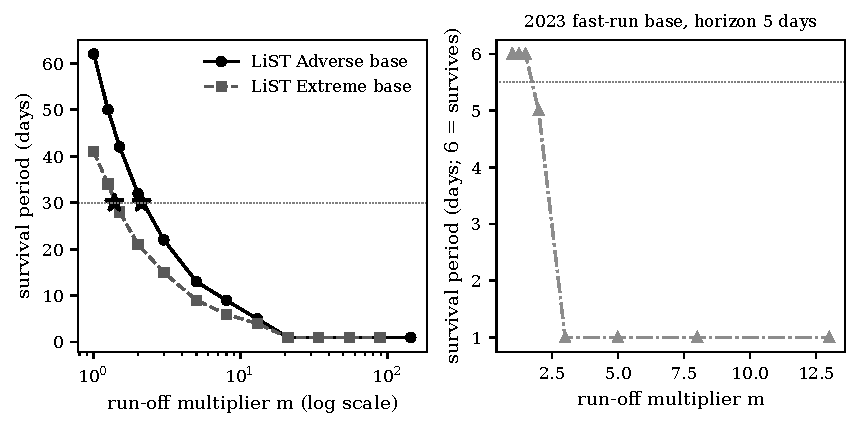
\includegraphics[width=0.98\textwidth]{sp-curve}
\caption{Survival period against the run-off multiplier on the three committed bases of case C16: the LiST Adverse and Extreme bases on the left with the thirty-day target as a dotted line and the threshold multipliers marked by stars, and the 2023 fast-run base on the right with its five-day ladder, on which a survival period of 6 stands for surviving the horizon.}
\label{fig:sp-curve}
\end{figure}

\Cref{fig:sp-curve} shows why the integer survival period is a poor object to invert. On the Adverse base it falls from \spAdv{} days at $m=1$ to 32 days at $m=2$ and 22 days at $m=3$, so the grid of the case design brackets the target between 2 and 3 and does not locate it; the solver returns \mAdv{}. On the fast-run base the curve shows that the base survives the five days up to $m=1.5$, reaches day 5 at $m=2$ and day 1 at $m=3$, so a thirty-day target is meaningless on it: no survival period under thirty days can be told from surviving the ladder, and the refusal is the correct answer rather than a failure of the solver.

The solved multiplier depends on the target as \cref{prop:threshold} says. \Cref{fig:by-target} plots it against $T$ for the two LiST bases; it is non-increasing, defined up to a target of \tMaxAdv{} days on the Adverse base and \tMaxExt{} days on the Extreme base, and refused from the survival period of the base upwards. The dotted lines are the hyperbolic rule $\mathrm{SP}(1)/T$ of \cref{prop:hyperbolic}; at 30 days it gives \hypAdv{} on the Adverse base and \hypExt{} on the Extreme base, \hypAdvErr{}\,\% and \hypExtErr{}\,\% from the solved values.

\begin{figure}[htbp]
\centering
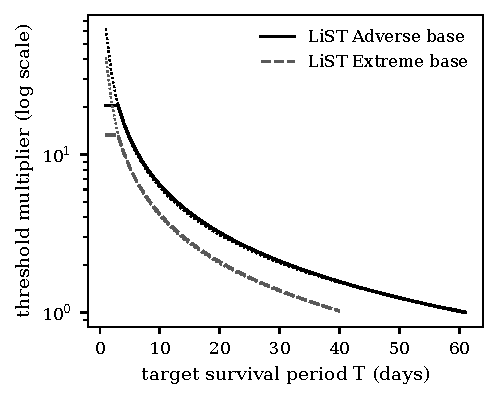
\includegraphics[width=0.6\textwidth]{by-target}
\caption{Threshold multiplier against the target survival period for the LiST Adverse and Extreme bases of case C16, on a logarithmic axis; the dotted lines are the hyperbolic rule equal to the survival period of the unscaled base divided by the target, and each curve ends at the largest target below the survival period of its base.}
\label{fig:by-target}
\end{figure}

\subsection{The corpus: solver against comparators}

The corpus has \kInst{} instances, \kSolved{} of which the oracle solves and \kRefused{} of which it refuses (\cref{tab:design}): \kHor{} because the target is not below the horizon, \kBase{} because the base already reaches it and \kUnr{} because no multiplier under the cap does.

\begin{table}[htbp]
\centering
\small
\setlength{\tabcolsep}{3pt}
\caption{Composition of the seeded corpus: 5 independent corpora of 1,000 synthetic banks, each solved at the targets of 2, 5, 10 and 30 days, counted by the outcome of the independent oracle.}
\label{tab:design}
\begin{tabular}{lr}
\toprule
Outcome of the oracle & Instances \\
\midrule
instances (banks $\times$ targets) & 20,000 \\
solved by the oracle & 8,568 \\
refused: target not below the horizon & 5,034 \\
refused: base survival period already at or below the target & 5,870 \\
refused: no multiplier under the cap reaches the target & 528 \\
solved, constant capacity and no inflow & 2,318 \\
solved, capacity on a monetisation schedule & 5,177 \\
\bottomrule
\end{tabular}
\end{table}


The engine's outcome equals the oracle's on every instance (H1: \kHOneDis{} disagreements). On the solved instances its multiplier exceeds the oracle's root by between \kHTwoMin{} and \kHTwoMax{} millionths, which is the rounding step, and every one satisfies the threshold property (H2). Panel A of \cref{tab:main-results} gives the comparison. The proposed solver answers none of the refused instances and leaves none of the solved ones without a number; its median relative error is \kPErr{}, about the rounding step, and it costs \kPEvals{} evaluations of the position on average. The scan of the case grid answers \kGFalse{}\,\% of the refused instances, because it returns the first grid point, 1, when the base already reaches the target; it finds no multiplier on \kGMiss{}\,\% of the solved ones; and its median relative error is \kGErrPc{}\,\%, with a 95th percentile of \kGErrQ{}. The finer grid cuts the median error to \kFErrPc{}\,\% at \kFEvals{} evaluations per solved instance and a median call of \kFTime{} ms against \kPTime{} ms for the solver. Brent's method on the survival period answers \kBFalse{}\,\% of the refused instances and returns a threshold on only \kBThr{}\,\% of the solved ones. The bisection without the refusal rule answers every refused instance, and returns a multiplier above the cap of the scenario on \kNBeyond{}\,\% of all instances.

\begin{figure}[htbp]
\centering
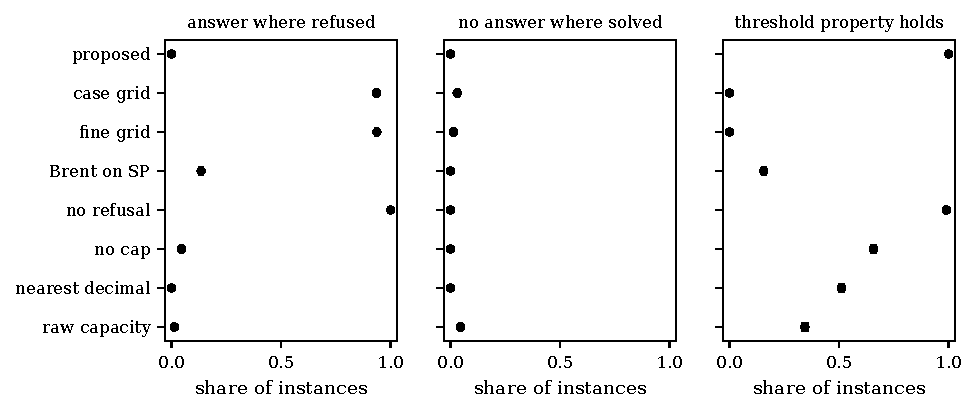
\includegraphics[width=0.98\textwidth]{methods}
\caption{Behaviour of the proposed solver and seven variants on the 20,000 instances of the corpus: from left to right the share of refused instances that are answered with a number, the share of solved instances left without an answer, and the share of solved instances whose multiplier is a threshold, each with a 95\% Wilson interval.}
\label{fig:methods}
\end{figure}

\Cref{fig:methods} shows the same three rates for all eight variants. Only the proposed solver is at 0, 0 and 1 together; the variants that remove one component differ from it in one of the three. The case grid overshoots the threshold by more than 10\% on \kHFour{}\,\% of the solved instances it answers, with a median overshoot of \kHFourMed{}\,\% and a 90th percentile of \kHFourQ{}\,\%, so H4 held. Brent's method returns a multiplier more than a millionth above the threshold on \kHFive{}\,\% of the solved instances, so H5 held: the interval on which the survival period equals the target is wide, and the root finder stops somewhere inside it.

H6 failed. On the solved instances with a constant capacity, no inflow and a finite base survival period, the multiplier $\mathrm{SP}(1)/T$ is within 10\% of the threshold on \kHSix{}\,\% of the instances, against the 80\% predicted, and the median relative error is \kHSixMed{}\,\%. \Cref{fig:scatter} shows the cause: with several segments of different rates the survival period of the unscaled run is set by the slow segments and the threshold by the fast ones, and the single-segment bounds of \cref{prop:hyperbolic} do not extend. On the committed bank the rule is within \hypAdvErr{}\,\% and \hypExtErr{}\,\%, close because one segment holds most of the deposits.

\begin{figure}[htbp]
\centering
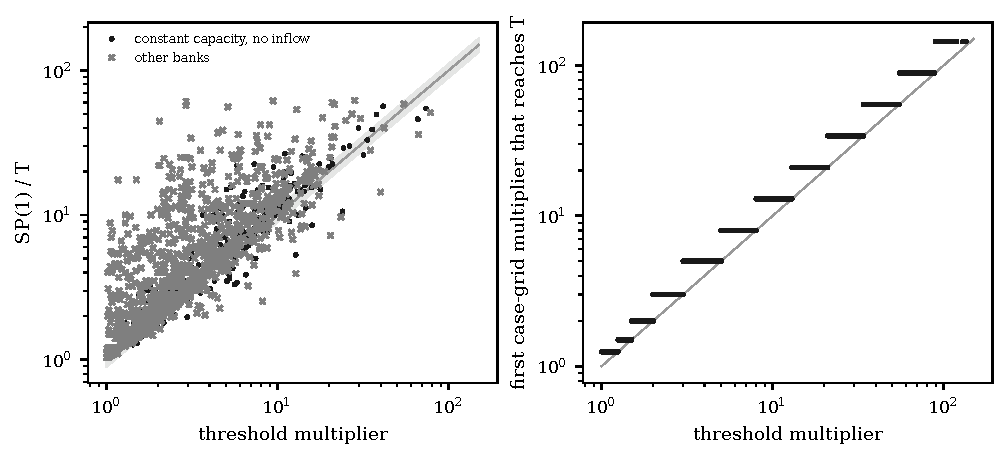
\includegraphics[width=0.98\textwidth]{scatter}
\caption{Left: the multiplier SP(1)/T against the oracle's threshold on a sample of 2,500 solved corpus instances, on logarithmic axes, with the identity line and a band of 10\%; banks with a constant capacity and no inflow are plotted as dots, the others as crosses. Right: the first multiplier of the case grid that reaches the target against the threshold, which lies above the identity line wherever the grid is coarse.}
\label{fig:scatter}
\end{figure}

\subsection{The round trip and the gap}

With a constant capacity and no inflow the survival period at the reported multiplier is exactly the target on \kHThreeMono{}\,\% of the \kFlat{} solved instances, as \cref{prop:roundtrip} states, and the sufficient condition of that proposition holds on all of them with a margin of at least \thErMarginMin{} (the outflow of day $T$ over $\delta Q_T$). With a monetisation schedule the survival period at the multiplier is below the target on \kHThreeGrow{}\,\% of the \kGrow{} solved instances, with a median gap of \kHThreeGapFifty{} days, a 90th percentile of \kHThreeGapNine{} days and a maximum of \kHThreeGapMax{} days (\cref{fig:gap}). H3 held in both clauses, the second by a wide margin. The gap is not a defect of the solver: the threshold property holds for every one of these instances. It is a property of capacity that grows, and it is the reason the method reports the survival period at the multiplier next to the multiplier.

\begin{figure}[htbp]
\centering
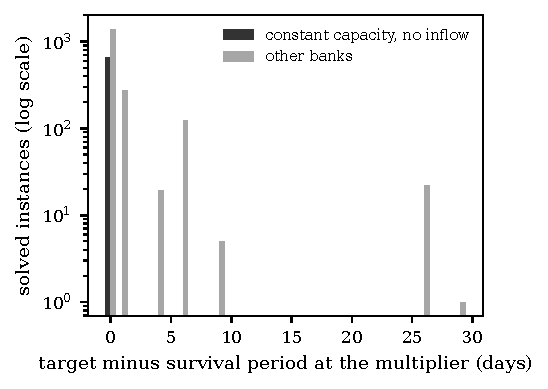
\includegraphics[width=0.6\textwidth]{gap}
\caption{Distribution of the gap between the target and the survival period at the reported multiplier over the solved corpus instances, separately for banks with a constant capacity and no inflow, where the gap is always zero, and for the other banks, where a growing capacity or an inflow can move the minimum of the window function to an earlier day.}
\label{fig:gap}
\end{figure}

On the committed fast-run base the same effect appears in a case the engine solves. With a target of 1, 2 or 3 days the multiplier is the same, \mTwo{}: the monetisation schedule releases capacity on days 1 to 3 and the survival period steps from \spBelowTwo{} days to day 1 across one decimal of the multiplier, so no multiplier gives a survival period of exactly 2 or 3. A target of 4 days is solved at \mFour{} with a survival period of 4, and a target of 5 days, equal to the horizon, is refused.

\subsection{Conventions and sensitivity}

The threshold moves with the capacity as \cref{prop:sensitivity} predicts. At the Adverse multiplier the critical day is day \dayZeroAdv{}, the elasticity of the multiplier with respect to the capacity is \elastAdv{}, and the derivative of \cref{eq:sensitivity} differs from the central difference of repeated solves by \derivRelAdv{}\,\% on the Adverse base and \derivRelExt{}\,\% on the Extreme base, within the 1\% of H7. Handing the solver the capacity schedule alone, without the inflows and the flows outside the segments, changes the Adverse multiplier from \mAdv{} to \rawAdv{} and the Extreme one from \mExt{} to \rawExt{}, \rawAdvPct{}\,\% on the Adverse base.

\begin{table}[htbp]
\centering
\small
\setlength{\tabcolsep}{3pt}
\caption{Sensitivity of the threshold multiplier at a target of 30 days to the conventions of case C16: the haircut band of 0.05, the immediate and slow monetisation schedules, the placement of the uninsured balance, and the three corners of the joint band that use the slow schedule; the last column is the survival period at the multiplier, which is the target wherever the round trip is exact and falls short of it where the slow schedule turns the threshold into a step; a refusal is stated, never a number.}
\label{tab:band}
\begin{tabular}{lrrr}
\toprule
Convention changed & Multiplier & Change (\%) & SP at $m^\ast$ \\
\midrule
\multicolumn{4}{l}{\textit{LiST Adverse base, central multiplier 2.118175}} \\
haircut low & 2.229711 & +5.3 & 30 \\
haircut high & 1.946672 & -8.1 & 30 \\
monetisation immediate & 2.118175 & +0.0 & 30 \\
monetisation slow & refused & & \\
uninsured as operational deposits & 2.796956 & +32.0 & 30 \\
uninsured as other legal entities & refused & & \\
joint: haircut low and slow monetisation & 1.063646 & -49.8 & 4 \\
joint: haircut central and slow monetisation & refused & & \\
joint: haircut high and slow monetisation & refused & & \\
\multicolumn{4}{l}{\textit{LiST Extreme base, central multiplier 1.383141}} \\
haircut low & 1.456144 & +5.3 & 30 \\
haircut high & 1.270925 & -8.1 & 30 \\
monetisation immediate & 1.383141 & +0.0 & 30 \\
monetisation slow & refused & & \\
uninsured as operational deposits & 1.936593 & +40.0 & 30 \\
uninsured as other legal entities & refused & & \\
joint: haircut low and slow monetisation & refused & & \\
joint: haircut central and slow monetisation & refused & & \\
joint: haircut high and slow monetisation & refused & & \\
\bottomrule
\end{tabular}
\end{table}


\Cref{tab:band} gives the effect of each convention. Moving every haircut by 0.05 changes the Adverse multiplier to \hcLowAdv{} (up \hcLowAdvPct{}\,\%) or \hcHighAdv{} (down \hcHighAdvPct{}\,\%). The slow monetisation schedule, which releases 25\% of the capacity on day 1 and all of it by day 10, lowers the capacity inside the window so far that the base survival period falls to \slowSpAdv{} days on the Adverse base and \slowSpExt{} days on the Extreme base, below the target of 30, and the solver refuses both. Mapping the uninsured balance to operational deposits raises the Adverse multiplier to \opAdv{} and the survival period of the base to \opSpAdv{} days. Mapping it to other legal entities, whose rate is 1 on day 1, makes the base survival period \legalSp{} day, and the solver refuses, as H9 predicted. The joint band does not keep the multiplier within 25\%: over the \jointSolvedAdv{} of nine combinations of haircut and monetisation that remain solved, the Adverse multiplier runs from \jointMinAdv{} to \jointMaxAdv{}, a deviation of \jointDevAdv{}\,\% from the central value, and H8 failed. The multiplier is stable to the haircut band alone and undefined, not unstable, under the slow schedule.

\begin{figure}[htbp]
\centering
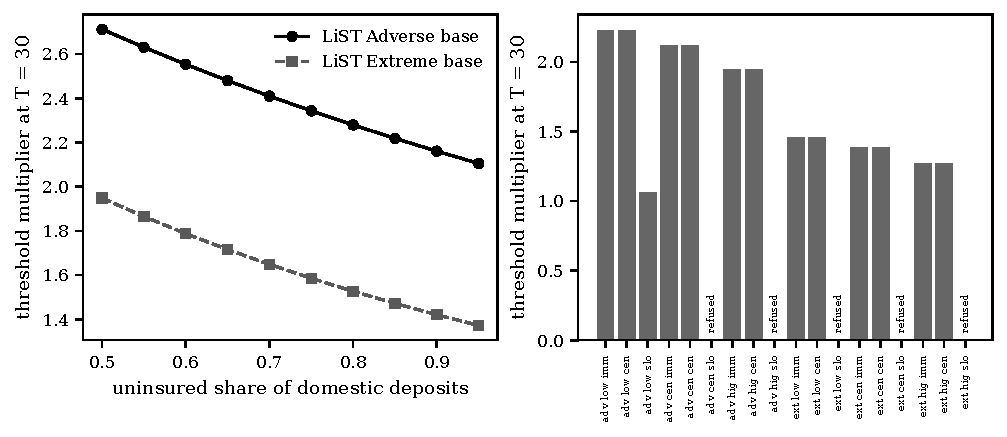
\includegraphics[width=0.98\textwidth]{band}
\caption{Threshold multiplier of the LiST Adverse and Extreme bases at a target of 30 days: on the left against the uninsured share of domestic deposits from 0.5 to 0.95, and on the right for the nine combinations of the haircut band and the immediate, central and slow monetisation schedules, with a refusal marked where the base already reaches the target.}
\label{fig:band}
\end{figure}

The multiplier also falls as the uninsured share rises (\cref{fig:band}, left): on the Adverse base it is \uninsLowAdv{} at a share of 0.5 and \uninsHighAdv{} at 0.95, since more of the deposit base sits in the segment with the faster rate and less run-off acceleration is needed to exhaust the capacity.

\subsection{The labelled run}

\begin{table}[htbp]
\centering
\small
\setlength{\tabcolsep}{3pt}
\caption{The fast-run base calibrated on the Table A.1 rows dated before 2023 and scored on the rows of the run: the modelled cumulative outflow share at the horizon of each row, its ratio to the observed share and the light of the case design (green from 0.8, amber from 0.5); rows with a horizon beyond the 5-day ladder are not scored.}
\label{tab:labelled-run}
\begin{tabular}{lccccc}
\toprule
Row & Days & Observed & Modelled & Ratio & Light \\
\midrule
SVB 2023 (scored) & 2 & 0.85 & 0.1708 & 0.201 & red \\
First Republic 2023 & 90 & 0.57 & beyond the 5-day ladder & -- & -- \\
SVB UK 2023 (scored) & 1 & 0.30 & 0.1263 & 0.421 & red \\
Credit Suisse 2023 & 90 & 0.21 & beyond the 5-day ladder & -- & -- \\
Signature 2023 (scored) & 1 & 0.20 & 0.1263 & 0.631 & amber \\
Icesave 2008 & 75 & 0.20 & beyond the 5-day ladder & -- & -- \\
Northern Rock 2007 (calibration) & 4 & 0.20 & 0.2528 & 1.264 & green \\
WaMu 2008 & 10 & 0.10 & beyond the 5-day ladder & -- & -- \\
IndyMac 2008 & 14 & 0.08 & beyond the 5-day ladder & -- & -- \\
\bottomrule
\end{tabular}
\end{table}


\Cref{tab:labelled-run} scores the fast-run base. Calibrated on the four rows dated before 2023, its rate is \rateMax{} per day, taken from the Northern Rock row; scored on the 2023 rows with horizons inside the ladder, it models \svbModel{} of the deposit base in the two days of the run against the observed 0.85, a ratio of \svbRatio{} and a red light. Against the second denominator of the case, the 140 billion dollars of outflow over the call-report deposits, which give a realised share of \depShare{}, the ratio is \depRatio{}. The two one-day rows are \ukRatio{} (red) for the sister bank in the United Kingdom, with \ukModel{} modelled against 0.30, and \sigRatio{} (amber) for the other failed bank of 2023. The in-sample row of Northern Rock is modelled at \nrModel{}, a ratio of \nrRatio{}. H10 failed: the base does not reach the amber bar at the event horizon.

The shortfall is not an artefact of the calibration rule. Replacing the maximum implied rate by the median (\rateMed{}) or the mean (\rateMean{}) lowers the ratio to \medRatio{} and \meanRatio{} (H12 held). The maximum itself rests on one row: leaving out Northern Rock leaves the maximum at \looNr{}, the rate of the WaMu row, and the other three leave-one-out fits return \rateMax{}.

\begin{figure}[htbp]
\centering
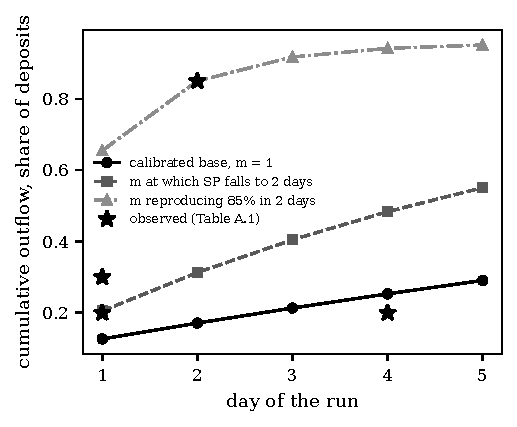
\includegraphics[width=0.6\textwidth]{labelled-run}
\caption{Modelled cumulative outflow, as a share of deposits, over the five days of the fast-run ladder at three multipliers of the calibrated rates, the calibrated base, the multiplier that brings the survival period to two days and the multiplier of the labelled run, against the observed rows of Table A.1 whose horizon lies inside the ladder, marked by stars.}
\label{fig:labelled-run}
\end{figure}

The reverse stress turns the shortfall into a distance. \Cref{fig:labelled-run} shows that the multiplier at which the modelled outflow reaches 0.85 in two days is \mSvb{}, against a cap of \capFast{} on the fast-run base, and that at this multiplier the survival period is one day. The multiplier that merely brings the survival period of the base to two days is \mTwo{}, so the multiplier of the labelled run is \ratioLab{} times larger and H11 held. In the model, the observed run lay far beyond the point at which the capacity is exhausted: a calibrated base that is red against the observation is not a base that is safe, because it takes a multiplier of \mTwo{} to exhaust its capacity. Both statements are about a synthetic bank.

\subsection{Outcome of every prediction}

\begin{table*}[htbp]
\centering
\small
\setlength{\tabcolsep}{3pt}
\caption{Reproductions and predictions with the value each one took. R1 to R5 restate values committed before the design document named them; H1 to H12 were written into a file whose modification time precedes that of the three result files (\cref{sec:experimental-design}). Three predictions failed (H6, H8, H10): the hyperbolic rule, the stability of the Adverse multiplier over the joint convention band, and the amber bar of the labelled run.}
\label{tab:hypotheses}
\begin{tabular}{lp{4.6cm}p{3.0cm}p{3.4cm}l}
\toprule
Id & Statement & Criterion & Measured & Outcome \\
\midrule
R1 & reproduction & Adverse multiplier 2.118175 & 2.118175 & reproduced \\
R2 & reproduction & Extreme multiplier 1.383141 & 1.383141 & reproduced \\
R3 & reproduction & fast run refused at 30 days & refused & reproduced \\
R4 & reproduction & modelled 2-day loss 0.17083 & 0.17083 & reproduced \\
R5 & reproduction & round trip of the threshold & SP 30, just below 31 & reproduced \\
H1 & outcome equals the oracle's & 0 disagreements & 0 of 20,000 & held \\
H2 & threshold within the rounding step & 0 to $10^{-6}$ above the root & 0.000 to 1.000 $\times10^{-6}$ & held \\
H3 & exact round trip: flat capacity; schedule & $\ge$99\%; $\ge$5\% with a gap & 100.0\%; 28.9\% & held \\
H4 & case grid overshoots by more than 10\% & $\ge$30\% of the solved instances & 75.7\% answered, 73.4\% all & held \\
H5 & Brent on SP misses the threshold & $\ge$10\% of solved & 82.6\% & held \\
H6 & SP(1)/T within 10\% of the threshold & $\ge$80\%, flat capacity & 42.7\% & failed \\
H7 & derivative equals finite difference & within 1\% & 0.0045\% & held \\
H8 & Adverse multiplier within 25\% over the band & $<$25\% & 49.8\% & failed \\
H9 & uninsured as legal entities: refusal & refused & refused & held \\
H10 & 2-day outflow reaches the amber bar & ratio $\ge$0.5 & 0.201 & failed \\
H11 & labelled multiplier $\ge2\times$ that bringing SP to 2 days & $\ge$2 & 4.58 & held \\
H12 & other calibration rules stay below amber & ratio $<$0.5 & 0.131 & held \\
\bottomrule
\end{tabular}
\end{table*}


\Cref{tab:hypotheses} lists the reproductions and predictions with the value each took. Nine of the twelve predictions held; H6, H8 and H10 failed. The failures bear on different parts of the method: the quick rule of H6 is not a substitute for the solver once several segments are present, the Adverse multiplier of H8 is not insensitive to the joint conventions, and the calibrated base of H10 does not reproduce the speed of the March 2023 run. The predictions that held are the ones that concern the solver itself, its agreement with the oracle, its threshold, its round trip and its comparison with the scans; the ones that failed concern what the committed bank and the calibrated run do. The reproductions R1 to R5 are not predictions and are not counted among the twelve.

\section{Ablation}
\label{sec:ablation}

The proposed solver has five components: the cap on the scaled rates of \cref{eq:scaled}, the refusal rule of \cref{eq:refuse-horizon,eq:refuse-base,eq:refuse-unreachable}, the continuous window function of \cref{eq:window}, the upward rounding with the neighbour check of \cref{eq:rounding}, and the effective capacity that folds the inflows and the flows outside the segments into $C_t$. \Cref{tab:ablation} removes one at a time on the \kInst{} instances of the corpus and scores the variant against the oracle with the metrics of \cref{eq:metrics}.

\begin{table*}[htbp]
\centering
\small
\setlength{\tabcolsep}{3pt}
\caption{Ablation on the corpus of 20,000 instances: each row removes one component of the proposed solver; the columns are the share of refused instances answered with a number, the share of solved instances left without a number, the share of solved instances whose multiplier is a threshold, the share of all instances answered with a multiplier above the cap, and the median relative error.}
\label{tab:ablation}
\begin{tabular}{p{4.4cm}p{1.9cm}p{1.9cm}p{1.9cm}p{1.9cm}p{1.9cm}}
\toprule
Variant & answer if refused (\%) & no answer if solved (\%) & threshold (\%) & beyond cap (\%) & median rel. error \\
\midrule
proposed solver (all components) & 0.0 & 0.0 & 100.0 & 0.00 & 8.9e-08 \\
without the cap on the scaled rates & 4.6 & 0.0 & 65.7 & 2.04 & 2.3e-07 \\
without the refusal rule & 100.0 & 0.0 & 99.0 & 3.48 & 9.2e-08 \\
without the continuous window function (Brent on SP) & 13.5 & 0.0 & 15.7 & 0.00 & 6.3e-02 \\
without upward rounding and the neighbour check & 0.0 & 0.0 & 51.1 & 0.00 & 4.6e-08 \\
without inflows and flows outside the segments & 1.4 & 4.6 & 34.4 & 0.00 & 1.5e-02 \\
\bottomrule
\end{tabular}
\end{table*}


Removing the cap leaves the solver able to answer where no admissible multiplier exists. The variant searches up to a multiplier of 1,000 with rates $m\,q_{j,d}$ that may exceed 1, and a rate above 1 turns the stock factor $1-q$ negative, so the stock changes sign and the cumulative outflow is no longer a share of the opening balance. It answers \kUFalse{}\,\% of the refused instances, and it returns a multiplier above the cap on \kUBeyond{}\,\% of all instances. Its multipliers are not thresholds of the model: they satisfy the threshold property on \kUThr{}\,\% of the solved instances, and the experiment did not isolate which of the artefacts of rates above 1 causes the failures. The cap is not a numerical convenience. It is what makes the scaled scenario a run-off scenario.

Removing the refusal rule leaves a bisection on a fixed bracket that always answers. It answers all \kRefused{} refused instances with an endpoint of its bracket, and on \kNBeyond{}\,\% of all instances the endpoint lies above the cap of the scenario, so the number it reports cannot be reached by any admissible run. Where it solves, it is as accurate as the proposed solver (median relative error \kNErr{}) and satisfies the threshold property on \kNThr{}\,\% of the solved instances; the cost is \kNEvals{} evaluations against \kPEvals{}, because a bisection does not use the shape of the function. The component is therefore not about accuracy. It decides whether a number is a result.

Removing the continuous window function means applying Brent's method to the integer survival period. The variant cannot bracket a target that the base already reaches or that no multiplier reaches, since $\mathrm{SP}(m)-T$ then has no sign change, and it answers \kBFalse{}\,\% of the refused instances where a sign change happens to exist. On the solved instances it returns a threshold on \kBThr{}\,\% only, because it stops inside the interval on which the survival period equals the target; its median error is \kBErrPc{}\,\%, and its 95th percentile \kBErrQ{}. The window function removes exactly that flat region.

Removing the upward rounding and the neighbour check, so that the root is rounded to the nearest decimal, keeps the refusals and the accuracy, with a median error of \kRErr{}, and fails the threshold property on about half of the solved instances: it satisfies it on \kRThr{}\,\%. The reason is the one in \cref{prop:threshold}: the set of multipliers that reach the target is open at the root, so a rounded-down value does not reach it. The check is cheap, and it gives the reader a number that reproduces.

Removing the effective capacity hands the solver the capacity schedule alone. It answers \kWFalse{}\,\% of the refused instances and fails to answer \kWMiss{}\,\% of the solved ones, since the position it solves is not the position of the ladder. On the instances that have inflows or flows outside the segments (\kRawFlowsN{} solved ones) the median error of its multiplier is \kRawFlows{}\,\%, and on the committed bank it moves the Adverse multiplier from \mAdv{} to \rawAdv{} and the Extreme one from \mExt{} to \rawExt{}. A reverse stress that is solved on a position other than the ladder's is a reverse stress of another bank.

Each component protects against a different failure: the cap against infeasible scenarios, the refusal rule against numbers for undefined targets, the window function against flat regions of the survival period, the rounding against a multiplier that does not reach the target, and the effective capacity against a position that differs from the ladder's. No single component carries the result; the proposed solver is the only variant at zero false answers, zero misses, no multiplier above the cap and the threshold property on every solved instance.

\section{Discussion}
\label{sec:discussion}

\subsection{What the multiplier says and does not say}

A multiplier of \mAdv{} on the Adverse base says that, in this model of this bank, the daily run-off rates of the supervisory scenario would have to be about twice as fast for the survival period to fall from \spAdv{} days to 30. It says that the distance to the target is modest, and that the target is not a remote one. It does not say that a run twice as fast is likely or that the bank has that headroom: the deposit behaviour is synthetic, the mapping of the uninsured balance to a supervisory class is a convention, and the multiplier changes by \jointDevAdv{}\,\% across the joint band of conventions. The reverse stress is a measure of distance within a model, and its value to a validator is that it states the distance in the unit of the scenario rather than in days of survival, which differ in how fast they change: \cref{fig:sp-curve} shows that the survival period drops from 62 to 32 days between $m=1$ and $m=2$ and from 13 to 1 day between $m=5$ and $m=21$.

The sensitivity formula explains part of the stability. With an elasticity of \elastAdv{} the multiplier moves by about one and a half times the relative change in capacity, so a shift of 0.05 in every haircut applied to the securities, which changes the capacity by a similar share, moves the multiplier by \hcLowAdvPct{}\,\% or \hcHighAdvPct{}\,\%. The refusals are the more important sensitivity. The slow monetisation schedule and the mapping to other legal entities make the base reach 30 days at a multiplier of 1, and the solver says so instead of returning a multiplier of 1. A table of multipliers across conventions with a column of refusals is more informative than one without, because a refusal marks the convention at which the bank is already at the target.

\subsection{The labelled run}

The score of the fast-run base is red, and the result is not a calibration accident. The maximum implied rate comes from a single row, Northern Rock, and the median and the mean rules give lower ratios. The deeper reason is structural. The base is a constant daily rate on one segment calibrated on runs of 4 to 75 days, and the March 2023 run was a two-day event in which a concentrated uninsured deposit base left at an implied rate of 0.6127 per day. A constant rate fitted on slower runs cannot reproduce a run in which the speed was set by coordination among large depositors, which the empirical work on the run describes \citep{cipriani2024,iyerpuri2012}. The multiplier of the labelled run, \mSvb{} times the calibrated rate against a cap of \capFast{}, quantifies it: the observed run was in the model about \ratioLab{} times further than the multiplier that brings the survival period to at most two days.

What the paper does not claim is as important. The red light does not show that a better calibration rule exists, and the multiplier of the labelled run is not a forecast of the next run. The protocol shows how a stress family can be scored against an event without being calibrated on it, and it records that this family does not reach the event.

\subsection{Failure cases and negative results}

Three predictions failed. The hyperbolic rule of H6 holds for one segment (\cref{prop:hyperbolic}) and fails on a mixture, with a median error of \kHSixMed{}\,\% on the corpus; it is a quick check for a bank dominated by one segment and not a replacement for the solver. The joint stability of H8 failed because of the monetisation schedule: it is the schedule, not the haircut, that moves the base survival period under the target. At the central and high haircuts the slow schedule makes the Adverse base reach the target at a multiplier of 1 and the solver refuses; at the low haircut the base stays above the target, the multiplier is \lowSlowM{}, and the survival period at the multiplier is \lowSlowSp{} days against \lowSlowBelow{} one decimal below it, so the threshold is a cliff and not an undefined value. The whole deviation of \jointDevAdv{}\,\% comes from that corner. The amber bar of H10 failed because of the speed of the run. A fourth result was not predicted and bears on the use of the method: with the monetisation schedule of the case design the survival period of the fast-run base steps from 4 days to 1 across one decimal of the multiplier, so targets of 1, 2 and 3 days have the same multiplier. A reverse stress on a short ladder with a fast-releasing capacity is a statement about a step, and the survival period at the multiplier is the figure that tells it.

\subsection{Implications for validation practice}

A validator who receives a stress model with a table of survival periods under three scenarios can add a column that the paper's method makes available: the multiplier at which each scenario reaches the target the institution cares about, or the statement that it does not. The column does not replace the scenarios, it measures how far they are from the target in one unit. Three practices follow. A reverse stress result should be reported with the survival period at the multiplier and just below it, so that the reader can check the threshold. A refusal should be reported as a result with its reason, in the same table as the multipliers. And a comparison of stress scenarios by their survival periods should count a bank that survives the horizon as longer than any day, as the supervisory exercise does by reporting that the position stays positive; a scan over a coarse grid that returns the first passing point answers the refused instances with a number and, in the corpus, gives a median error of \kGErrPc{}\,\% on the instances it solves.

\section{Limitations}
\label{sec:limitations}

\subsection{Internal validity}

The oracle shares the model of the engine: it recomputes the position by the closed form of the stock and finds the root by bisection, so it tests the solver, the bracketing, the rounding and the refusal logic, and not the model. An error in the compounding model itself, for example a wrong treatment of a rate of 1, would be shared by both. The model is checked elsewhere in the product against the printed percentages of the supervisory note and against a day-by-day stock, which this paper does not repeat. The corpus is a plant: the three refusal reasons occur because it is built to produce them, and the rates of its segments are drawn from a distribution chosen by the author, so the shares in \cref{tab:main-results} describe that corpus, in which \kRefused{} of \kInst{} instances are refused, and not the frequency of refusals in practice. The comparators are those a validator would assemble from the forward tools; a more careful scan, with an adaptive grid, would close the gap to the proposed solver in accuracy and not in the handling of refusals. The corpus run took \kWallMin{} minutes, and the experiment was run on one machine, so the timings carry the load of that machine.

\subsection{External validity}

The committed bank is one bank, with real balance-sheet aggregates and synthetic behaviour, valued at one date. The deposit mapping, the monetisation schedule, the calendar and the calibration rule are conventions, and \cref{tab:band} shows that the answer depends on them. The base rates are the transcribed values of one supervisory exercise on a TARGET2 calendar, applied here on a United States business-day calendar. The labelled run is one event with three rows that fall inside the five-day ladder, and the other two 2023 rows have horizons of 90 days, beyond the ladder, so they are not scored. A score on three rows has no sampling interval; the two denominators of the observed outflow are the only uncertainty the paper reports for it. Nothing in the paper concerns what the failed bank did, and the multipliers are not its headroom. The corpus covers constant and two-phase rate paths on horizons of 5 to 125 days; rates that vary through the horizon in other ways, such as a path that accelerates late, are not generated, and the proposition on the exact round trip is not tested on them.

\subsection{Construct validity and scope}

The multiplier is a one-parameter family: it scales every segment by the same factor, so it cannot represent a run that concentrates on one segment. The cap makes the scenario a share but also means that a segment already at a rate of 1, such as the financial segment, does not contribute to the distance. The capacity is exogenous: a faster run does not change haircuts, collateral calls or the willingness of the central bank to lend, all of which a real run would move, and the position is evaluated at the end of the day, so intraday shortfalls are not seen. The target of 30 days is the example of the research that motivates the rung, not a regulatory threshold. The related work on reverse liquidity stress testing contains three book chapters that we could not read, so the novelty of the solver is limited to what this paper defines and measures, and the absence of a published multiplier with a refusal rule is unverified beyond the search made. Finally, the paper does not model run dynamics with a stochastic depositor process, which would give the survival period a distribution and the multiplier a meaning in probability.

\section{Reproducibility}
\label{sec:reproducibility}

The code, the committed documents of case C16 and every stored result are in the repository named in the header of the first page. All commands run from the repository root with \texttt{python} on the environment of the product (the \texttt{riskvalidation} package 1.1.0 with the market, machine-learning and stress extras, and the requirements of the case pipeline). The experiments read the committed documents of \texttt{data/derived/C16}; no raw data are needed, and no path of a machine is written in any file.

\begin{itemize}
\item \texttt{experiments/run\_reverse\_c16.py} rebuilds the three bases, calls the engine, and writes \texttt{results\_reverse\_c16.json} (reproductions, derivative, convention band, labelled run).
\item \texttt{experiments/run\_corpus.py} generates the five corpora from seeds 20261107 to 20261111, runs the oracle, the solver and the comparators, and writes \texttt{results\_corpus.json}; it took \kWallMin{} minutes on one machine with other jobs running (\kProc{}, Python \kPy{}).
\item \texttt{experiments/run\_theory.py} writes \texttt{results\_theory.json} from seed 20261120.
\item \texttt{experiments/hypotheses.json} holds the predictions and the dates at which they were written; \texttt{experiments/test\_core.py} and \texttt{experiments/test\_results.py} test the shared code and the stored results.
\item \texttt{make\_numbers.py}, \texttt{make\_tables.py} and \texttt{make\_figures.py} write \texttt{tables/numbers.tex}, the tables and the vector figures from the stored results, so that no number of the text is typed; \texttt{fetch\_references.py} writes \texttt{references.bib} from the records of the cited works.
\end{itemize}

The times in \cref{tab:main-results} are medians of measured calls, written by the experiment scripts to the stored results; they depend on the machine and are not a property of the method. The solve on the Adverse base takes \timeAdvMs{} ms and on the Extreme base \timeExtMs{} ms.

\section{Conclusions}
\label{sec:conclusions}

Reverse liquidity stress can be posed as the root of a continuous window function of a run-off multiplier, capped so that every rate stays a share, rounded up to six decimals, and refused with a reason when the target is not bracketed. On \kInst{} instances of a seeded corpus the engine implementing it agrees with an independent oracle on every outcome, returns a threshold on every solved instance (\kPThr{}\,\%) and answers none of the \kRefused{} refused ones, while a scan of the multiplier grid of the case design answers \kGFalse{}\,\% of them and overshoots the threshold by a median of \kGErrPc{}\,\%. Removing the cap, the refusal rule, the continuous window, the upward rounding or the effective capacity each breaks a different property.

On the bank of case C16 the multiplier that brings the survival period to 30 days is \mAdv{} on the Adverse base and \mExt{} on the Extreme base, and the 2023 fast-run base is refused because its ladder is shorter than the target. The fast-run base, calibrated only on rows dated before 2023, models \svbModel{} of the deposit base in the two days of the run against 0.85 observed, a ratio of \svbRatio{}, and the multiplier that reproduces the observation is \mSvb{} times the calibrated rate. The Adverse multiplier moves by \jointDevAdv{}\,\% over the joint band of conventions and is refused under the slow monetisation schedule. Nine of twelve predictions held; the hyperbolic rule, the stability over the joint band and the amber bar of the labelled run failed.

The next steps are to give the survival period a distribution through a stochastic depositor process and to report the multiplier as a quantile of that distribution, to extend the family beyond a common multiplier to segment-specific ones with a plausibility measure, and to repeat the labelled-run score on banks whose deposit behaviour is observed.


\bibliographystyle{plainnat}
\bibliography{references}

\end{document}
